\documentclass{article}

% if you need to pass options to natbib, use, e.g.:
% \PassOptionsToPackage{numbers, compress}{natbib}
% before loading nips_2016
%
% to avoid loading the natbib package, add option nonatbib:
% \usepackage[nonatbib]{nips_2016}

\PassOptionsToPackage{numbers,sort&compress}{natbib}
\usepackage[final]{nips_2016} % produce camera-ready copy

\usepackage[utf8]{inputenc} % allow utf-8 input
\usepackage[T1]{fontenc}    % use 8-bit T1 fonts
\usepackage{hyperref}       % hyperlinks
\usepackage{url}            % simple URL typesetting
\usepackage{booktabs}       % professional-quality tables
\usepackage{amsfonts}       % blackboard math symbols
\usepackage{nicefrac}       % compact symbols for 1/2, etc.
\usepackage{microtype}      % microtypography
\usepackage{graphicx}
\usepackage{subcaption}     % Add Subfigures and Subtables
\usepackage{multirow}

\title{Spotify Data Analysis}

% The \author macro works with any number of authors. There are two
% commands used to separate the names and addresses of multiple
% authors: \And and \AND.
%
% Using \And between authors leaves it to LaTeX to determine where to
% break the lines. Using \AND forces a line break at that point. So,
% if LaTeX puts 3 of 4 authors names on the first line, and the last
% on the second line, try using \AND instead of \And before the third
% author name.

\author{
  S2648988\\
  %% examples of more authors
  \And
  S2101527\\
 \And
  S2693506\\
  \And
  S1953043\\
}

\begin{document}

\maketitle
 \textit{}
% \section{Current progress}
% \begin{itemize}
%     \item Did some data cleaning in the form of:
%     \begin{itemize}
%         \item Assume that 'Song URL' column is not needed
%         all values are non-null, no need to remove rows
%         \item should change "Date" column type to datetime
%         \item sort dates in chronological order
%         \item could rename columns (standard variable names)
%         \item Scale the audio features to be in the range [0, 1]
%         \item Loudness: Log base 10 (of the absolute value) then divde by 60.
%     \end{itemize}
%     \item did some exploratory data analysis
%     \begin{itemize}
%         \item looked at the top 10 artists in terms of popularity (total points accumulated and number of songs that enetered the top 10)
%         \item line chart of how this top 10 changes over time
%     \end{itemize}
%     \item attempted multiple linear regression using audio features to predict popularity with poor results (3\% accuracy). This lead us to attempt to look at this question from a clasification approach.
%     \item Used web crawler to obtain the published date for each song
%     \item Used daily averaged audio features as the dataset and apply the Holt-Winters triple exponential smoothing algorithm (an optimized moving average algorithm with seasonal and trend features) to fit and predict the data.
%     \begin{itemize}
%         \item Used the K-fold method on our training dataset to train and test the model. Then, use two months of data as validation data.
%         \item Set the seasonal period to 7 days (one week), which is easily visible in the dataset. The predicted period is 30 days (one month).
%         \item The results show a mean error of 0.004 on the test data and a normalized mean square error of 0.00003 on the validation data (which is based on danceability).
%         \item The algorithm can predict the general trend for the following month.
%     \end{itemize}
% \end{itemize}

% \section{Plans for Completion}
% Two questions we chose to explore:
% \begin{itemize}
%     \item Can we figure out which artists or songs are going to be popular in 2024 given the historic data from 2017?
%     \begin{itemize}
%         \item Looking at this as a classification rather than regression problem - using Naive Bayes as a baseline?
%         \item Using Neural Network to predict better (recurrent)?
%     \end{itemize}
%     \item Are there any patterns in what day(s) of the week and/or months experience the most streams?
%     \begin{itemize}
%         \item Averaging audio features for different week days / months
%         \item Auto-correlation
%     \end{itemize}
% \end{itemize}

% Planned draft completion 17 Nov 2024



% \newpage

\begin{abstract}
This report explores three different questions in Hit Song Science: whether a song's popularity can be accurately predicted based on various audio features and artist information, whether audio features alone are effective predictors of songs that are more popular during weekends, and lastly whether we can predict the trend of each feature associated with popular songs over time. Well-known supervised learning algorithms were used for the first two, while other predictive models and neural networks were used for the third. Best performances were achieved by the decision tree, random forest, and Holt-Winters models respectively.
 
\end{abstract}

\section{Introduction}
Spotify is the world's largest streaming service for music worldwide with an estimated 640 million active users \cite{spotifyCompanyInfo}.
% https://newsroom.spotify.com/company-info/
Their charts, especially the global top 200, are of great importance as they show the most popular and relevant songs for any given day. These are of great importance to brands, record labels and the artists themselves as charting high and over longer periods of time can boost their careers or cement artists as being household names in the industry \cite{ariSpotifyCharts}. 
% https://aristake.com/how-to-rise-through-the-spotify-charts/
It is therefore interesting to explore whether any insights can be made into what determines a song’s popularity.
% swtich this and above senstences pot.
Numerous past examples of studies concerned with predicting song popularity have been found. Examples include work done by Harriman Samuel Saragih \cite{Indonesian-streaming} who used 13 classification algorithms to predict a song’s popularity using 12 audio features with the highest accuracy achieved being 0.697 and an F1-Score of 0.694. Other studies have done similar work taking genre popularity into account as well \cite{utwente}. 

Our work starts off with a similar classification task but also looks at other trends in popularity and musical aspects as well. Using data obtained from the Spotify global top 200 charts from 01/01/2017 until 29/05/2023, this paper investigates various facets of song popularity and attempts to investigate whether we can use machine learning models to a) make predictions about a song’s popularity, b) find what makes songs popular on weekends and c) predict future trends in music. Ultimately, we hope to achieve a comprehensive set of analyses for various questions such that anyone researching or analysing trends in music, whether for work or for pleasure, can make use of these results.


 % Alternative title suggestions: "What makes a song popular?", "Predicting music trends and song popularity"

 % Proposed question phrasing: 

 % % (1) Can we figure out which artists or songs are going to be  popular in 2024 given the historic data from 2017?
 % (1) Is it possible to predict future trends in song releases for 2024 based on historic data?

 % (2) Can musical aspects of a song alone be used to accurately predict a song's popularity?
 % (2) What aspects of a song determine its popularity?
 
 % -> weeday-weekend < yes
 
 % -> in general < no


\section{Exploratory data analysis}

The given dataset contains about 0.5 million instances of songs that have been a part of the “Top 200”  published globally between 2017 and 2023. It includes the song titles, information about the artists, song url, information in the form of scores for each song’s audio features as well as its popularity. 
% These points came from the reference dataset that scored a song between 1 and 200 depending on it placement on the charts, where placing first on the chart resulted in 200 points and placing 200th meant receiving one point.
The audio features describe different sonic characteristics of each song and are defined in detail on Spotify's website \cite{spotify_web}.


Irrelevant columns such as ‘Song URL’ were dropped. Other columns were renamed and dates were converted to datetime objects and their order reversed. The next step was to scale the audio features in the range of 0 to 1. 
% For loudness, the scaling was done to log base 10(of the absolute value)/60. 
The resulting dataset is the reference dataset to be used in the upcoming tasks.

% For the exploratory data analysis, we discarded the scores from 2023 as the data provided was of only the first half and performed the analysis on the data between the years 2017-2022. 


\begin{figure}[h]
    \centering
    \begin{subfigure}[b]{0.49\textwidth}
        \centering
        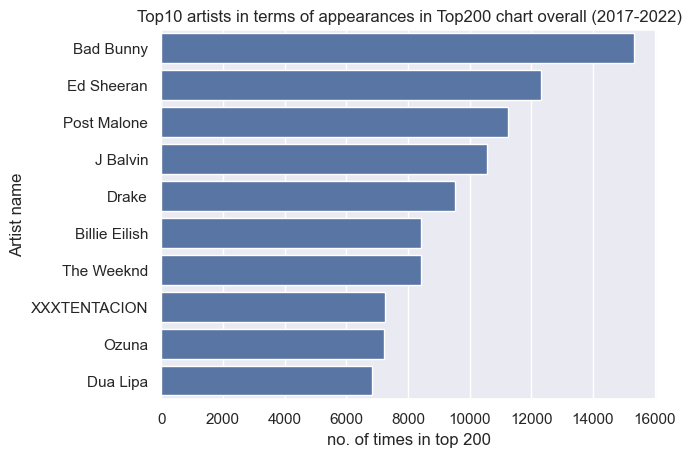
\includegraphics[width=\textwidth]{Figures/top10artist.png}
        \caption{Top 10 artists in terms of appearances}
        \label{fig:Top10artiststop}
    \end{subfigure}
    \hfill
    \begin{subfigure}[b]{0.49\textwidth}
        \centering
        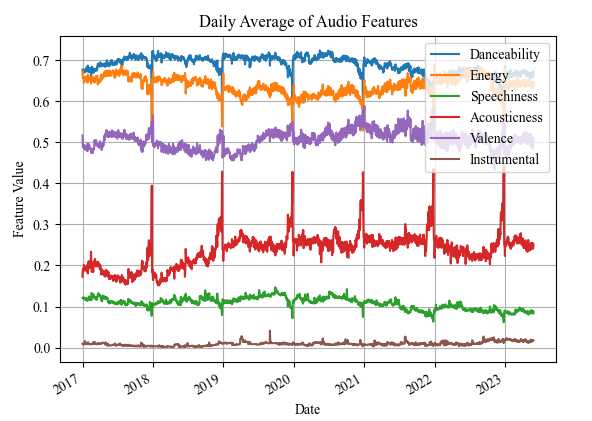
\includegraphics[width=\textwidth]{Mean}
        \caption{Daily average audio feature}
        \label{fig:Mean}
    \end{subfigure}
    \caption{Initial data visualisations}
    \label{fig:data_exploration}
\end{figure}

% \begin{figure}[htbp]
%     \centering
%     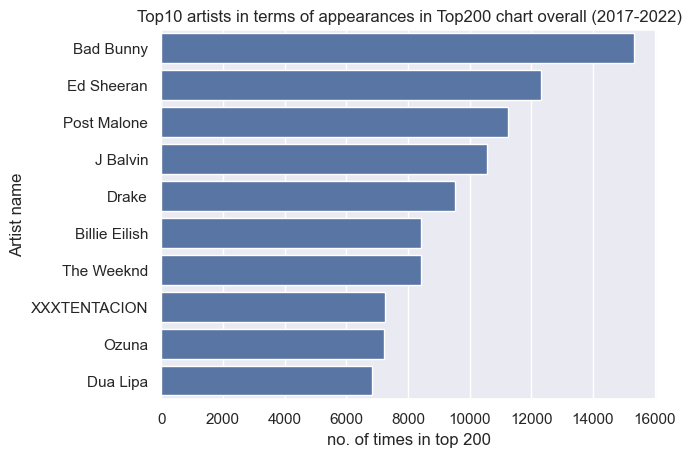
\includegraphics[width=0.5\linewidth]{Figures/top10artist.png}
%     \caption{Top 10 artists}
%     \label{fig:Top10}
% \end{figure}



% \begin{figure}[htbp]
%     \centering
%     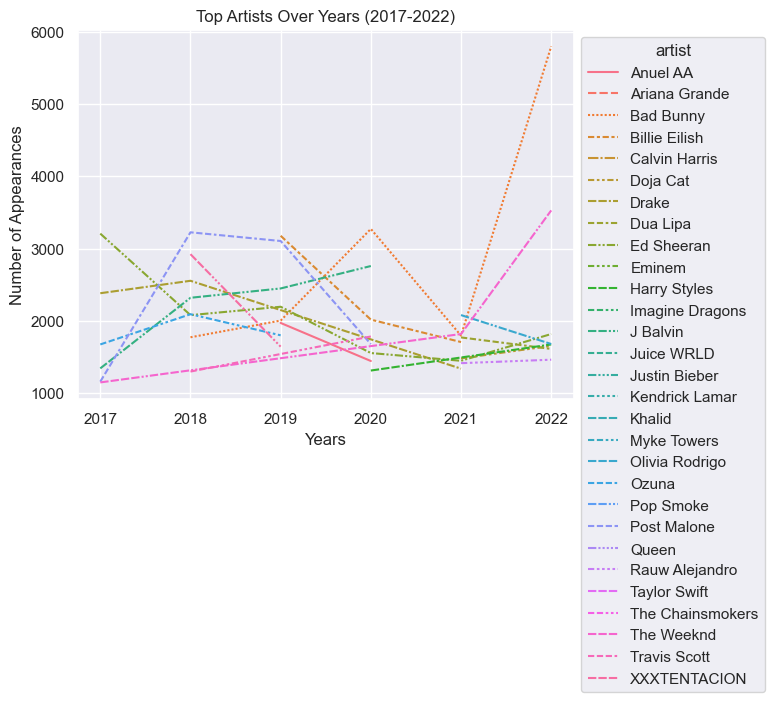
\includegraphics[width=0.5\linewidth]{Figures/topartistsongs.png}
%     \caption{Songs of top 10 artists per year}
%     \label{fig:Topartists}
% \end{figure}

Figure \ref {fig:Top10artiststop} shows the top 10 artists that have the highest number of appearances in the top 200 charts. Additionally, a separate visualisation is created showing the appearances of the top 10 artists for every year.
% specifically compiling the top 10 artists every year from 2017-2022 and how many songs each artist has in top 200 each year. 
This data is presented in Figure \ref{fig:Topartists} in the appendix. From the analysis done, we can see that certain artists have been consistently popular, with multiple songs in the top 200 every year. Another observation is that most of the artists in top 200 are from the USA which can imply that the location of an artist can play a part in their popularity as well.



\section{Task 1: Can we accurately predict a song's popularity?}
% This section compares 3 learning models to see which can most accurately classify popularity of a song.

\subsection{Data preparation}
An important aspect when creating the labels for the dataset was attributing the popularity classes to a song. To do this, the total points accumulated per song throughout its charting history were calculated. The songs were then annotated as being “high” popularity if they were in the top 25\% of songs ranked by total number of points, “low” popularity for being in the bottom quarter, and "medium" for being in the middle 50\%. Additionally, we ran the models on data with only high and low popularity for comparison.
% lnote: don't think this is clear

% This split was chosen as a compromise between not creating a large class imbalance while also accounting for the fact that splitting the dataset in half would not do any justice to the fact that the largest hits [APPENDIX XYZ]

Using audio features alone resulted in accuracies only marginally better than the baseline prediction.
% lnote: audio features alone to predict popularity. Could be placed at the end of this section.
Therefore, we opted to use other aspects provided in the dataset to predict popularity: artist popularity, artist nationality and number of collaborators on the track. The artist popularity was determined as the total points accumulated by the artist from 2017 to 2022. Similarly, the nationality score was determined by the frequency of that nationality in the chart in the same time frame. Lastly, the number of collaborators was determined by counting the number of artists collaborating on each track. The training set was the data from 2017 to 2022, and the 2023 data made up the test set.

\subsection{Learning Models}
Three supervised learning methods were chosen for this classification task: naive Bayes, logistic regression and decision tree. 
% why did I choose these
% parameters.

\textbf{Naive Bayes} (NB) is a generative model meaning it models every feature as normally distributed. Using these distributions it then 
% uses the formula below to predict the class for a particular input:
% \[
% P(C_k \mid x) = \frac{P(x \mid C_k) P(C_k)}{P(x)}
% \]
% Where \(C_k\) is the class and \(x\) is the feature being modelled. For all \(k\) classes, \(P(C_k \mid x\)) is calculated and the highest value 
determines the final class.
It assumes all features are independent given the class which means this model fails to recognise connections between features that may in fact rely on each other. It usually provides a good baseline due to its simplicity and good performance.


% the probability of the feature belonging to that class is calculated and the highest value ends up being the value chosen.
% \begin{itemize}
%     \item \(P(C_k \mid X)\) is the posterior probability of class \(C_k\) given the feature vector \(X\).
%     \item \(P(X \mid C_k)\) is the likelihood of \(X\) given class \(C_k\).
%     \item \(P(C_k)\) is the prior probability of class \(C_k\).
%     \item \(P(X)\) is the evidence, which is the probability of the feature vector \(X\) across all classes.
% \end{itemize}

% For the Naïve Bayes assumption (features are conditionally independent given the class), the likelihood \(P(X \mid C_k)\) can be written as:

% \[
% P(X \mid C_k) = \prod_{i=1}^n P(x_i \mid C_k)
% \]

% where \(x_i\) are the individual features of \(X\).


\textbf{Logistic Regression} (LR) is a discriminative classifier meaning it tries to distinguish between classes rather than modelling each class individually. It weights every feature in terms of how indicative it is of predicting a certain class. It is a probabilistic classifier and the supervised learning method as is naive bayes. 
% In its most simple form, logistic regression can be represented with the formula below:
% \[
% P(y=c\mid \mathbf{x}) = \sigma(\mathbf{w}^\top \mathbf{x})
% \]
% Where \(\mathbf{w}\) is the weights vector, \(\mathbf{x}\) is the vector feature vector and \(\sigma(z)\) is the sigmoid function used to make the final value be between 0 and 1.
Logistic regression does not make an independence assumption and therefore can outperform naive bayes when there are many correlated features.

\textbf{Decision Tree} (DT) is a supervised learning method that continuously divides up the feature space to categorise new input. It effectively creates a tree-like structure where every node contains a decision that defines a boundary between classes. To classify unseen data, one follows a path along the tree leading to a leaf node which will result in the predicted class. Decision trees have the benefit of being able to classify non-linear data and are easily interpretable because of their intuitive nature. 

\subsection{Results}
Table \ref{tab:lea_model_comparison} shows the final accuracy and F1 scores for the three models chosen. Although having similar accuracy for two popularity classes, the F1 scores for the NB and LR models are quite low. Only the DT model achieves a score of over 0.7. Additionally, the DT model clearly outperforms the other two in terms of accuracy and the F1 score when popularity is divided into three classes.

\begin{table}[htbp]
    \centering
    \small
    \caption{Model performance comparison for classifying popularity}
    \label{tab:lea_model_comparison}
    \begin{tabular}{lcccc}
        \toprule
        \multirow{2}{*}{Model} & \multicolumn{2}{c}{2 popularity classes} & \multicolumn{2}{c}{3 popularity classes} \\
        \cmidrule(lr){2-3} \cmidrule(lr){4-5}
         & Accuracy & F1 Score & Accuracy & F1 Score \\
        \midrule
        Naive Bayes & 0.672 & 0.575 & 0.358 & 0.344 \\
        Logistic Regression & 0.659 & 0.582 & 0.555 & 0.419 \\
        Decision Trees & 0.790 & 0.774 & 0.732 & 0.705 \\
        \bottomrule
    \end{tabular}
\end{table}

From the confusion matrix in Figure \ref{fig:lea_confusion}, we can see the correctly and mistakenly classified classes for the best-performing model as found in Table \ref{tab:lea_model_comparison}. In the case where there were two popularity classes (0 being ``low" and 1 being ``high") we can see that although the model rarely predicts a class ``high" to a low popularity song, it incorrectly predicts the class for a high popularity song around half of the time. In the case where there were three popularity classes there are also many incorrect predictions made, especially for the ``low" (labelled 0) and ``high" (labelled 2) popularity classes which are both most often mistaken with the ``medium" popularity class.

\begin{figure}[htbp]
    \centering
    \begin{subfigure}[b]{0.38\textwidth}
        \centering
        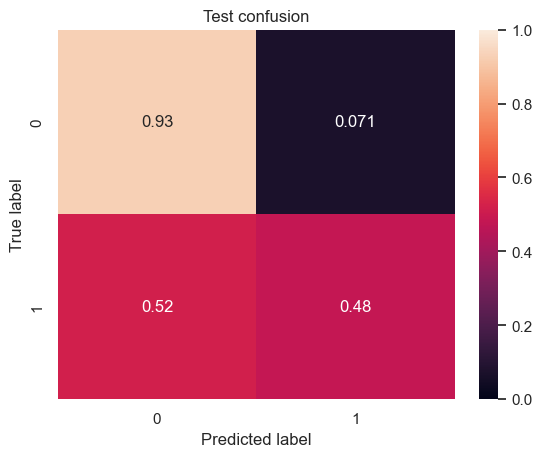
\includegraphics[width=\textwidth]{Figures/2classes_confusion.png}
        \caption{2 popularity classes}
        \label{fig:left}
    \end{subfigure}
    \hfill
    \begin{subfigure}[b]{0.38\textwidth}
        \centering
        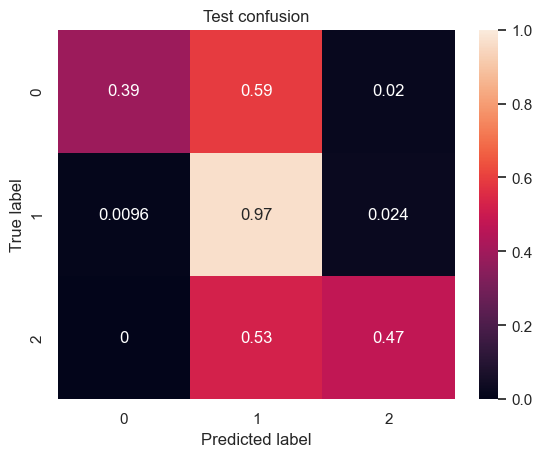
\includegraphics[width=\textwidth]{Figures/3classes_confusion.png}
        \caption{3 popularity classes}
        \label{fig:right}
    \end{subfigure}
    \caption{Confusion matrices for popularity classification using the decision tree model}
    \label{fig:lea_confusion}
\end{figure}

% The results suggest that moderate success at classifying a song's popularity for two with worse performance for three popularity classes. The chosen features might not be indicative enough to determine whether a song is likely going to reach the lower 100 of the chart and drop off fairly quickly or reach a higher placement and chart for longer periods of time.
% % Due to time constraints, no additional data was added alongside the data provided. 
% Improvements could be made by using additional audio features such as mode or tempo that can be accessed using the Spotify Web API [CITE].
% % [CITE] as previous work has shown that these features in [CITE] and [CITE] or with 
% Additional information such as album statistics and streams could be used and it would be interesting to examine how an artist's profile impacts the popularity of a song. 
% %Using more advanced models alongside some additional features

\section{Task 2: What makes some songs more popular on weekends?}

\subsection{Learning Models}

It can also be meaningful to ask what features, if any, make specific songs more popular on weekends than weekdays. This section attempts to answer this question using just the audio features and well-known supervised learning models. In addition to the three methods introduced in the first task, this task utilises two new supervised learning models: K-Nearest Neighbours and Random Forest.

\textbf{K-Nearest Neighbours} (KNN) is an elegant classification algorithm that assigns classes to data points based on the classes of the k data points nearest to it \cite{a2024_16}. For our purposes, the model uses euclidean distance and a decision threshold of $0.5$. \textbf{Random Forest} (RF) forms an ensemble of $n$ trees fitted to various subsets of the dataset and takes averages to make predictions \cite{a2018_sklearnensemblerandomforestclassifier}. Again, we use the default $0.5$ decision threshold.
% maybe give more detailed descriptions?

\subsection{Data Preparations}

This task required a new dataset with song titles as rows, 7 features columns, as well as a target column with binary entries: 1 if the song is more popular on weekdays, 0 otherwise. The audio features were averaged from the reference dataset so that each row contained one unique song, yielding a dataset of size (7457, 8). Each song was classified as follows. First, a separate dataset was created with songs as rows, dates from 01/01/2017 to 29/05/2023 as columns, and the total popularity points gained by each songs on each day as the entries. The columns were then separated into weekdays (Mon-Thurs) and weekends (Fri-Sun), and the points were averaged accordingly. Songs with a higher number of average points on weekdays than that of weekends were classified as 1, and vice versa.

This resulted in a binary dataset with a class imbalance: 4442 instances of 1 and 3015 instances of 0. To prevent bias towards the dominant class, the dataset was balanced out via oversampling, where random instances of 0 were duplicated until the classes were equal. Oversampling was chosen over weight modification as there is no meaningful cost difference between the two classes. 

\subsection{Methods}

\begin{figure}[htbp]
\centering
\begin{minipage}{.5\textwidth}
  \centering
  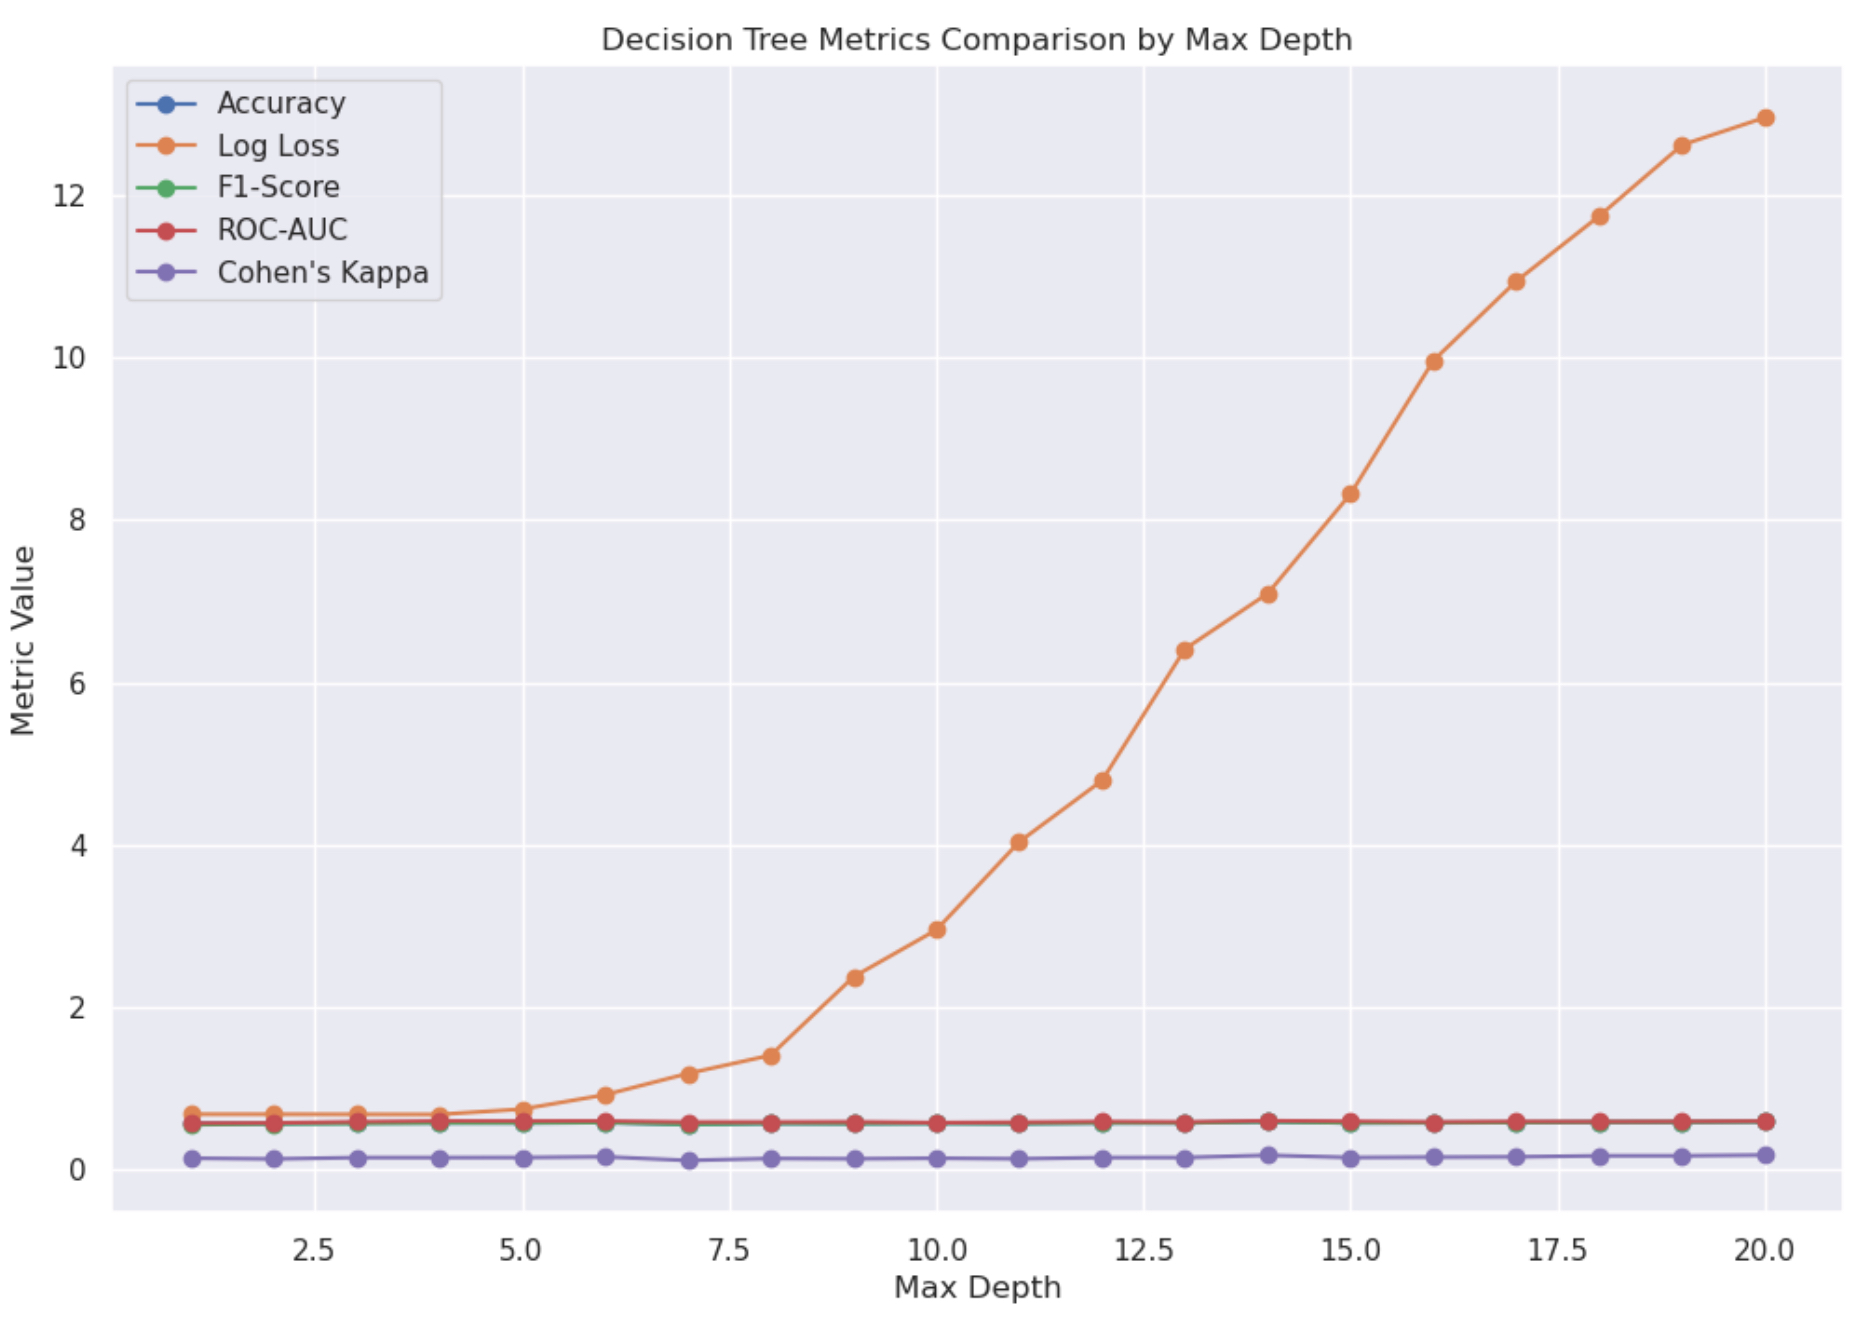
\includegraphics[width=.9\linewidth]{Figures/DT_hyperparameter.png}
\end{minipage}%
\begin{minipage}{.5\textwidth}
  \centering
  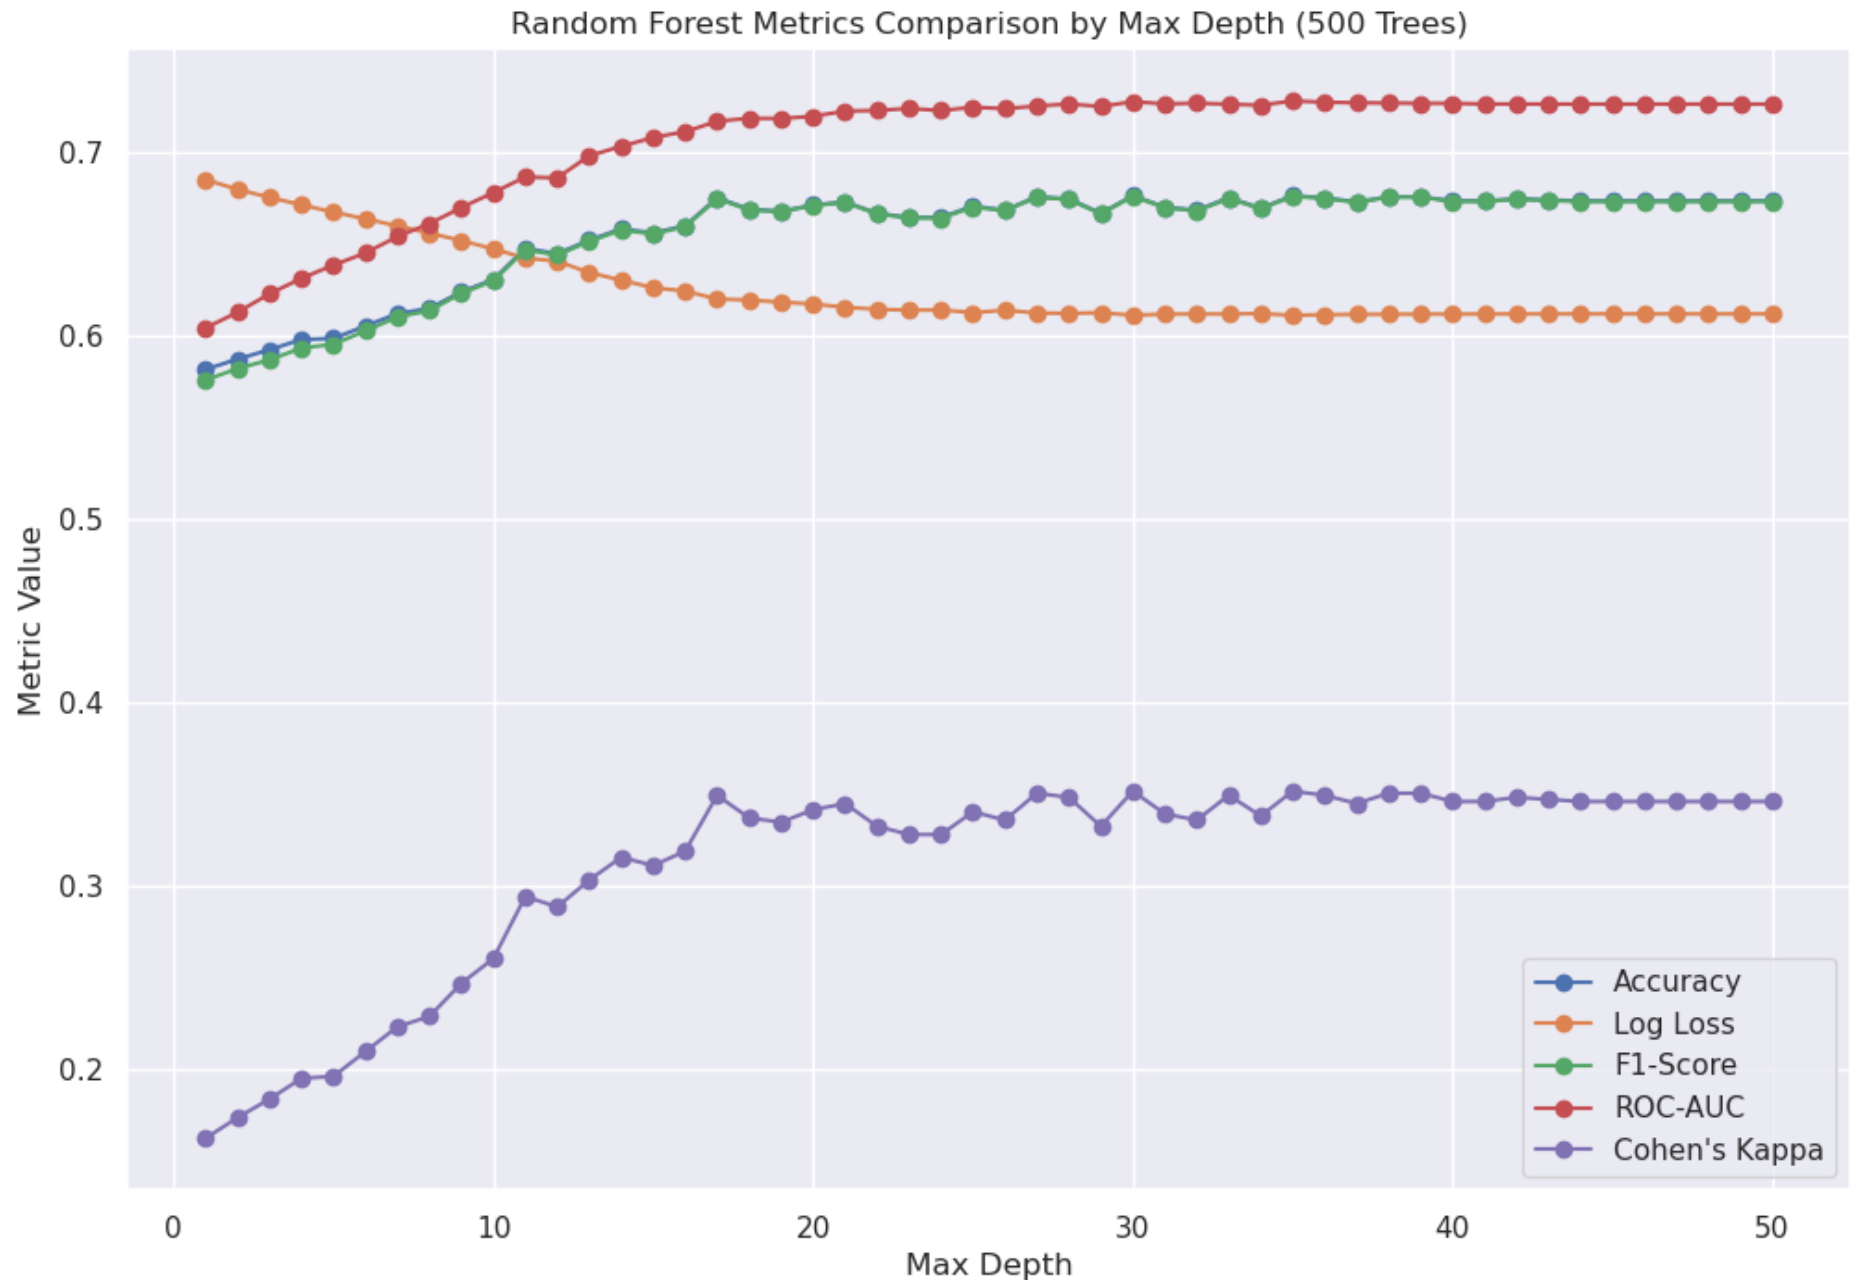
\includegraphics[width=.9\linewidth]{Figures/RF_max_depth.png}
\end{minipage}
\caption{Plots displaying the performances of the DT and RF classifiers for varying hyper-parameter values.}
\label{fig:hyperparameter}
\end{figure}

Choosing the right hyper-parameter values is crucial for obtaining accurate predictions. To this end, each classification model was trained on a train set (0.8) then tested on the corresponding test set for a range of hyper-parameter values and compared using the following well-known metrics: accuracy, logarithmic loss, f1-score, ROC-AUC, and Cohen's Kappa. Figure \ref{fig:hyperparameter} displays the effects of varying the hyper-parameters of the DT and RF classifiers respectively. For both models, the accuracy increases initially and then slowly approaches a maximum. However, the generalisation logarithmic loss rapidly increases after a depth of 4 for the DT classifier, while it decreases and then seems to approach a minimum for the RF classifier. Thus the depths of 4 and 43 were chosen for the DT and RF classifiers respectively. In similar manner, the number of nearest neighbours for the KNN classifier was chosen to be 30. The full analysis can be found in the appendix in Figure \ref{fig:hyperparameter_table}. Other parameters were found to have negligent effect.

% \subsection{Cross-validation}


\textbf{K-fold cross validation} makes $k$ unique train-test partitions of the dataset rather than just one. Averaging the $k$ predictions provides us with more accurate generalisation performances than the standard train-test split. But since the train-test split proportions vary with $k$, one must be cautious when choosing its value. To fix the value of $k$, the accuracy and variance of each model was compared for different values of $k$, and the k-values that yielded high accuracy and low variance were chosen: 6 for NB, 8 for KNN, 5 for LR, 5 for DT, and 10 for RF. The full analysis can be found in the appendix in Figures \ref{fig:validation_plot} and \ref{fig:validation_table}.

\subsection{Results and Evaluation}

\begin{table}[htbp]
\centering
\small
\caption{Table comparing the performances of each model}
\label{tab:Results}
\begin{tabular}{lrrrrr}
\toprule
{} &     Naïve Bayes &     Logistic Regression &    KNN &     Decision Trees &     Random Forest \\
\midrule
Accuracy      & 0.5580 & 0.5662 & 0.5803 & 0.5646 & 0.6741 \\
ROC-AUC  & 0.7461 & 0.6814 & 0.6779 & 0.6962 & 0.6060 \\
F1 Score & 0.5509 & 0.5662 & 0.5791 & 0.5629 & 0.6791 \\
log loss & 0.5852 & 0.5913 & 0.6133 & 0.5983 & 0.7336 \\
Cohen's kappa  & 0.1163 & 0.1327 & 0.1607 & 0.1308 & 0.3484 \\
MSE      & 0.4420 & 0.4338 & 0.4197 & 0.4354 & 0.3259 \\
\bottomrule
\end{tabular}
\end{table}


The prediction performances of each model for their chosen hyper-parameter values and validation folds is displayed in Figure \ref{tab:Results}. The RF classifier stands out as the most accurate by far compared to the others in all metric. This is perhaps expected as the dataset is highly complex and non-linear. The poor performance of the NB classifier can be explained by the fact that in reality the features are far from independent of each other: high danceability correlates with high valence, and so on. 

Further insight can be gained by examining the confusion matrices associated with each of the models in Figure \ref{fig:cm} in the appendix. Interestingly, while the KNN classifier provides a higher overall accuracy than both the DT and LR classifiers, the latter two outperform the former when it comes to correctly predicting songs that are more popular on weekends. The RF classifier not only has the highest accuracy, but also produces the most balanced predictions. 

Intuitively, one may expect stronger correlations between a song's audio features and its popularity during weekends. Nevertheless, each model does outperform the baseline majority classifier, implying that the song features are good enough indicators of whether a song will be more popular on weekdays or weekends. The plots in Figure \ref{fig:Importances} in the appendix suggest that valence, the measure of "musical positiveness" of a song, is the feature with the biggest contribution. This is in agreement with the common conception that cheerful, euphoric songs are enjoyed more on weekends than weekdays. 




% \section{Learning methods}
% 2 pages   

% \section{Results}
% 1.5 pages

% Section


\section{Task 3: Predicting the Future Trend}
\subsection{Time Series Algorithm}

Time series forecasting is an analytical approach that examines data changing over time, using statistical models to predict future patterns and trends.  Through this analysis, researchers can spot and understand patterns in time-based data, revealing both the direction and magnitude of changes.


\textbf{Holt-Winters Method}, also known as triple exponential smoothing, is a time series forecasting technique that accounts for both trend and seasonality\cite{winters}. The algorithm uses three factors: $\alpha$ for data smoothing, $\beta$ for trend smoothing, and $\gamma$ for seasonal change smoothing. After experimentation, we select the Nelder-Mead method as the optimal convergence technique to find the best parameters. Given that audio features exhibit trend or seasonal characteristics, the Holt-Winters method is well-suited for predicting these features. 


\textbf{Long Short-Term Memory (LSTM)} is a type of recurrent neural network (\textbf{RNN}) designed to address the vanishing gradient\cite{vanish_gradient} problem often faced by traditional RNNs. An LSTM unit consists of a cell and three gates: input, output, and forget. This structure enables LSTMs to selectively retain or discard information over extended sequences, making them highly effective for tasks requiring long-term context. 

\subsection{Metrics}
To predict the future trend of song genres, it's crucial to understand the future trends of audio features. To measure these trends, we calculate the average value of each audio feature on a daily basis. Since songs on the Top 200 list are already popular enough to represent trends, we don't consider ranks when calculating the average data. We can clearly see seasonal patterns and Christmas patterns (spikes in acousticness) in the mean values (shown in Figure \ref {fig:Mean}), indicating that it can be a good representation of trends. 

Given the inherent uncertainty in real-world scenarios, we've opted to predict trends for the upcoming week. This timeframe strikes a balance between a substantial forecasting period and reasonable prediction accuracy. We utilize daily average data from 1/1/2022 to 31/12/2022 for our training and test datasets. For the Holt-Winters method, we employ an 6-fold cross-validation approach. We set the season length to 30 days and the prediction length to 7 days in trainings and same settings in validations. For LSTM, we divide the data into training and testing sets with a 10:1 ratio and use Mean Squared Error (MSE) to train the model and the Adam optimizer to update each parameter. For validation, we use one month of consecutive data from 2023 to predict the following week's data. We conduct 112 such validations and use the mean value of the mean square error (MSE) of these validations as our final metric.

\subsection{Results}
We evaluate the prediction accuracy using the average Mean Squared Error (MSE) of the validation dataset (from 2023). The results in Table \ref {tab:predict_model_comparison} show that both algorithms perform well in predicting trends over a one-week timeframe, with MSE levels of $10^{-5}$ . Holt-Winters outperforms LSTM in Danceability, Energy, Speechiness, and Acousticness, while LSTM excels in Instrumental and Valence—particularly Instrumental. Notably, Holt-Winters shows superior performance for features with more pronounced periodic characteristics, highlighting the importance of trend and seasonal factors in the algorithm for future predictions. Our chosen season length (30 days) and prediction period (7 days) appear reasonable. Another advantage of Holt-Winters is its ability to predict 7 days at once, allowing us to use a week's data to train the model. This approach aligns better with our validation data settings. LSTM performs better for Instrumental and Valence due to its long-term memory capabilities, enabling good results even without obvious patterns. Considering these results and the computational cost of each algorithm (LSTM being significantly more resource-intensive), we conclude that Holt-Winters is the preferable method for predicting audio features for any upcoming week.

\begin{table}[htbp]
    \centering
    \small
    \caption{Model performance comparison for Holt-Winters and LSTM}
    \label{tab:predict_model_comparison}
    \begin{tabular}{lcccc}
        \toprule
        \multirow{2}{*}{Features} & \multicolumn{2}{c}{Average Mean Square Error (MSE)} \\
        \cmidrule(lr){2-3} 
         & Holt-Winters($\times 10^{-5}$) & LSTM($\times 10^{-5}$) \\
        \midrule
        Danceability & 2.021 & 5.265 \\
        Energy & 3.542 & 5.540 \\
        Speechiness & 1.265 & 4.432 \\
        Acousticness & 8.5 & 13.2  \\
        Instrumental & 0.729 & 0.361\\
        Valence & 6.872 & 6.542\\
        \bottomrule
    \end{tabular}
\end{table}



\section{Conclusions}

\textbf{Popularity prediction:} The results suggest that moderate success at classifying a song's popularity for for ``high" vs ``low" popularity with worse performance for three popularity classes. The chosen features might not be indicative enough to determine whether a song is likely going to reach the lower 100 of the chart and drop off fairly quickly or reach a higher placement and chart for longer periods of time.
% Due to time constraints, no additional data was added alongside the data provided. 
Improvements could be made by using additional audio features such as mode or tempo that can be accessed using the Spotify Web API \cite{spotify_web}.
% [CITE] as previous work has shown that these features in [CITE] and [CITE] or with 
Information such as album statistics and streams could also be used and it would be interesting to examine how an artist's profile impacts the popularity of a song. 
%Using more advanced models alongside some additional features

\textbf{Weekday vs Weekend:} Although the results are reasonably satisfactory, it is important to acknowledge that improvements could be made through various means. For example, a more comprehensive set of data which is not restricted to just the top 200 songs of each day would be a better fit for this type of prediction. Also, arguments for more sensible ways of categorising the songs into the two classes can be made. Lastly, a more thorough analysis involving adjustments to the confidence thresholds of the models used as well as the implementation of more complex machine learning models could improve the overall accuracy of the predictions.

\textbf{Audio Feature Prediction:} Our analysis reveals that both Holt-Winters and Long Short-Term Memory (LSTM) methods demonstrate high efficacy in trend prediction with mean MSE in $10^{-5}$ level. The Holt-Winters method shows a slight advantage for most features( Danceability, Energy, Speechiness, and Acousticness) and offers the added benefit of reduced computational requirements.  However, LSTM may demonstrate higher accuracy when additional data (such as rankings and artist information) is incorporated into the training input.


\newpage

% \section{Instructions}

% The report should use this template and be 6 pages in length. Do not change the fontsize or layout. It should be compilable with pdflatex.

% Structuring the text as follows is recommended, but not mandatory.

% \begin{itemize}
% \item Introduction
%   \begin{itemize}
%   \item description of the task/objective
%   \item relevant background and related previous work
%   \begin{itemize}
%       \item "Predicting song popularity based on Spotify’s audio features: insightsfrom the Indonesian streaming users" by Harriman Samuel Saragih
%       \item "Prediction of product success: explaining song popularity by audio features from Spotify data" by Nijkamp, Rutger
%       \item "Predicting Music Popularity Using Music Charts" by Carlos Vicente Soares Araujo
%   \end{itemize}
%   \item explanation of the significance/relevance of the objective/task
%   \end{itemize}
% \item Data preparation
% \item Exploratory data analysis
% \item Learning methods
% \item Results
% \item Conclusions
% \end{itemize}

% \section*{Citations and References}
% You can manage your bibliography---adding citations and references to other work---through BibTeX.
% Please see \url{https://www.overleaf.com/learn/latex/Bibliography_management_with_bibtex} for guidance.

% We show a minimal example of how to use it here.

% \LaTeX{} \cite{latex2e} is a set of macros built atop \TeX{} \cite{texbook}.

\section*{Statements of contribution}
\begin{itemize}
    \item \textbf{s2101527:} Responsible for Task 2 and abstract.
    \item \textbf{s1953043:} Responsible on task 1 and the introduction. Started data exploration.
    \item \textbf{s2648988:} Responsible for Task 3. Started data exploration.
    \item \textbf{s2693506:} Responsible for Exploratory Data Analysis. Started LSTM in Task 3.

\end{itemize}

\bibliography{refs.bib}
\bibliographystyle{ieeetr}

\section{Appendix}
 \begin{figure}[htbp]
     \centering
     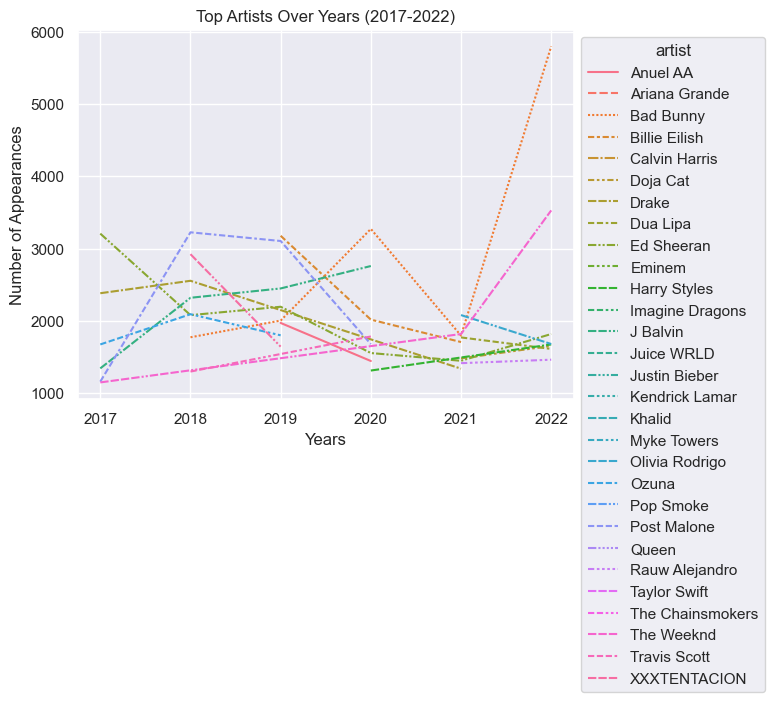
\includegraphics[width=0.7\linewidth]{Figures/topartistsongs.png}
     \caption{Songs of top 10 artists per year}
     \label{fig:Topartists}
 \end{figure}
 
% \begin{figure}[htbp]
%     \centering
%     \begin{subfigure}[b]{0.4\textwidth}
%         \centering
%         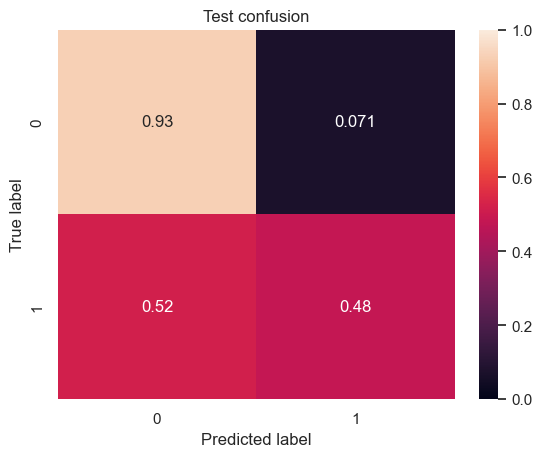
\includegraphics[width=\textwidth]{Figures/2classes_confusion.png}
%         \caption{2 popularity classes}
%         \label{fig:left}
%     \end{subfigure}
%     \hfill
%     \begin{subfigure}[b]{0.4\textwidth}
%         \centering
%         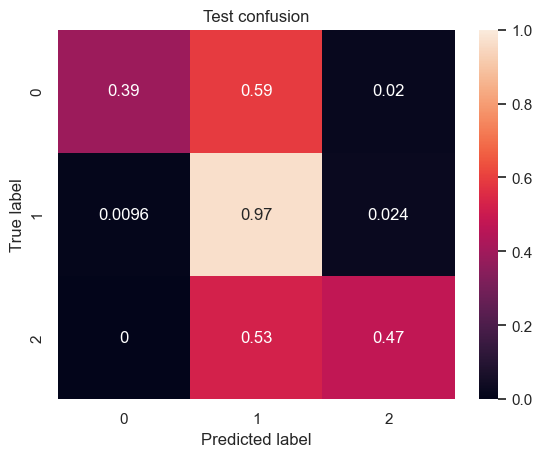
\includegraphics[width=\textwidth]{Figures/3classes_confusion.png}
%         \caption{3 popularity classes}
%         \label{fig:right}
%     \end{subfigure}
%     \caption{Confusion matrices for popularity classification using the decision tree model}
%     \label{fig:lea_confusion}
% \end{figure}

% \begin{figure}[h]
%     \centering
%     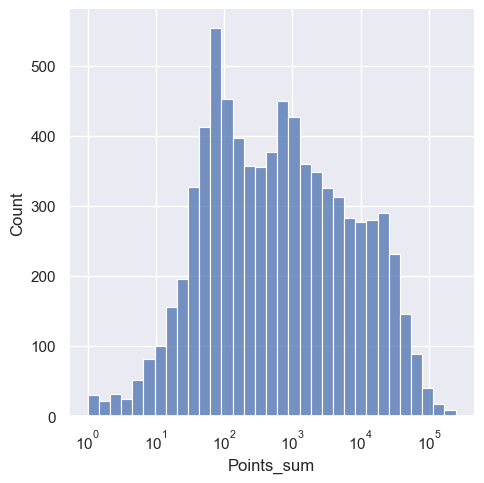
\includegraphics[width=0.5\textwidth]{Figures/dist_points_sum.png} % Replace 'example-image' with your image filename
%     \caption{Histogram showing the number of occurrences for songs at various total points}
%     \label{fig:distribution-of-song-popularity}
% \end{figure}



\begin{figure}[htbp]
\centering
\begin{minipage}{1\textwidth}
  \centering
  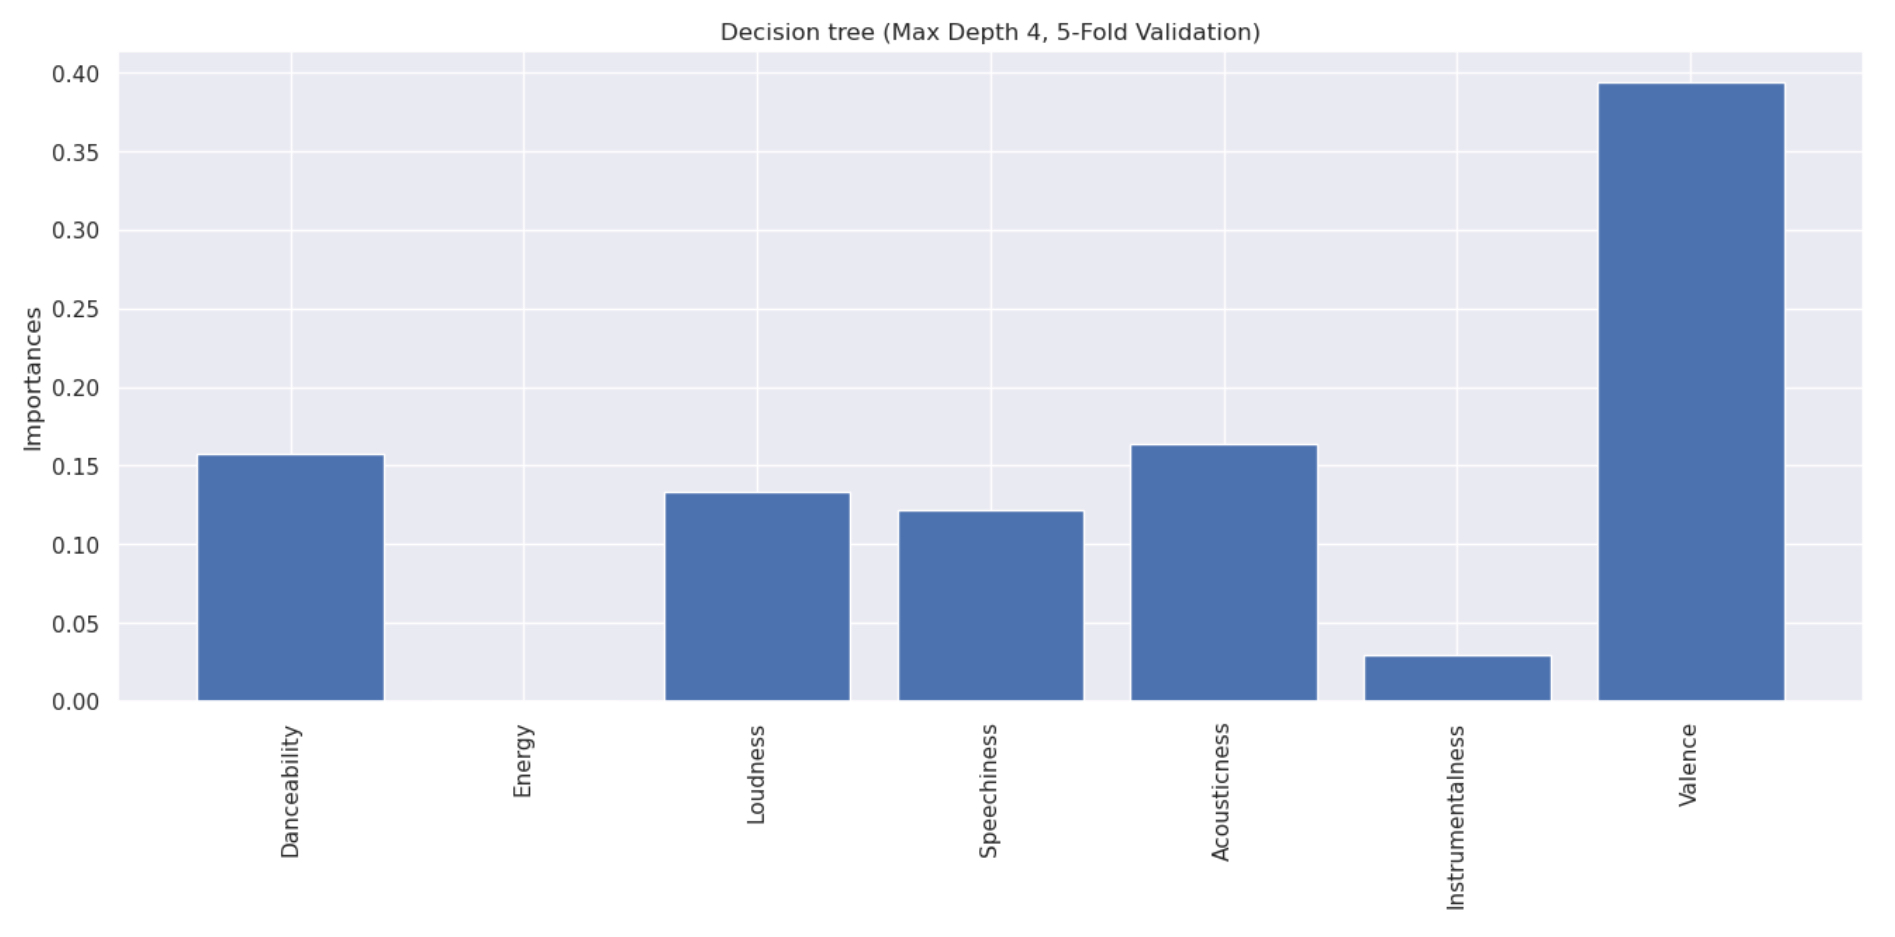
\includegraphics[width=1\linewidth]{Figures/DT_importances.png}
\end{minipage}
\begin{minipage}{1\textwidth}
  \centering
  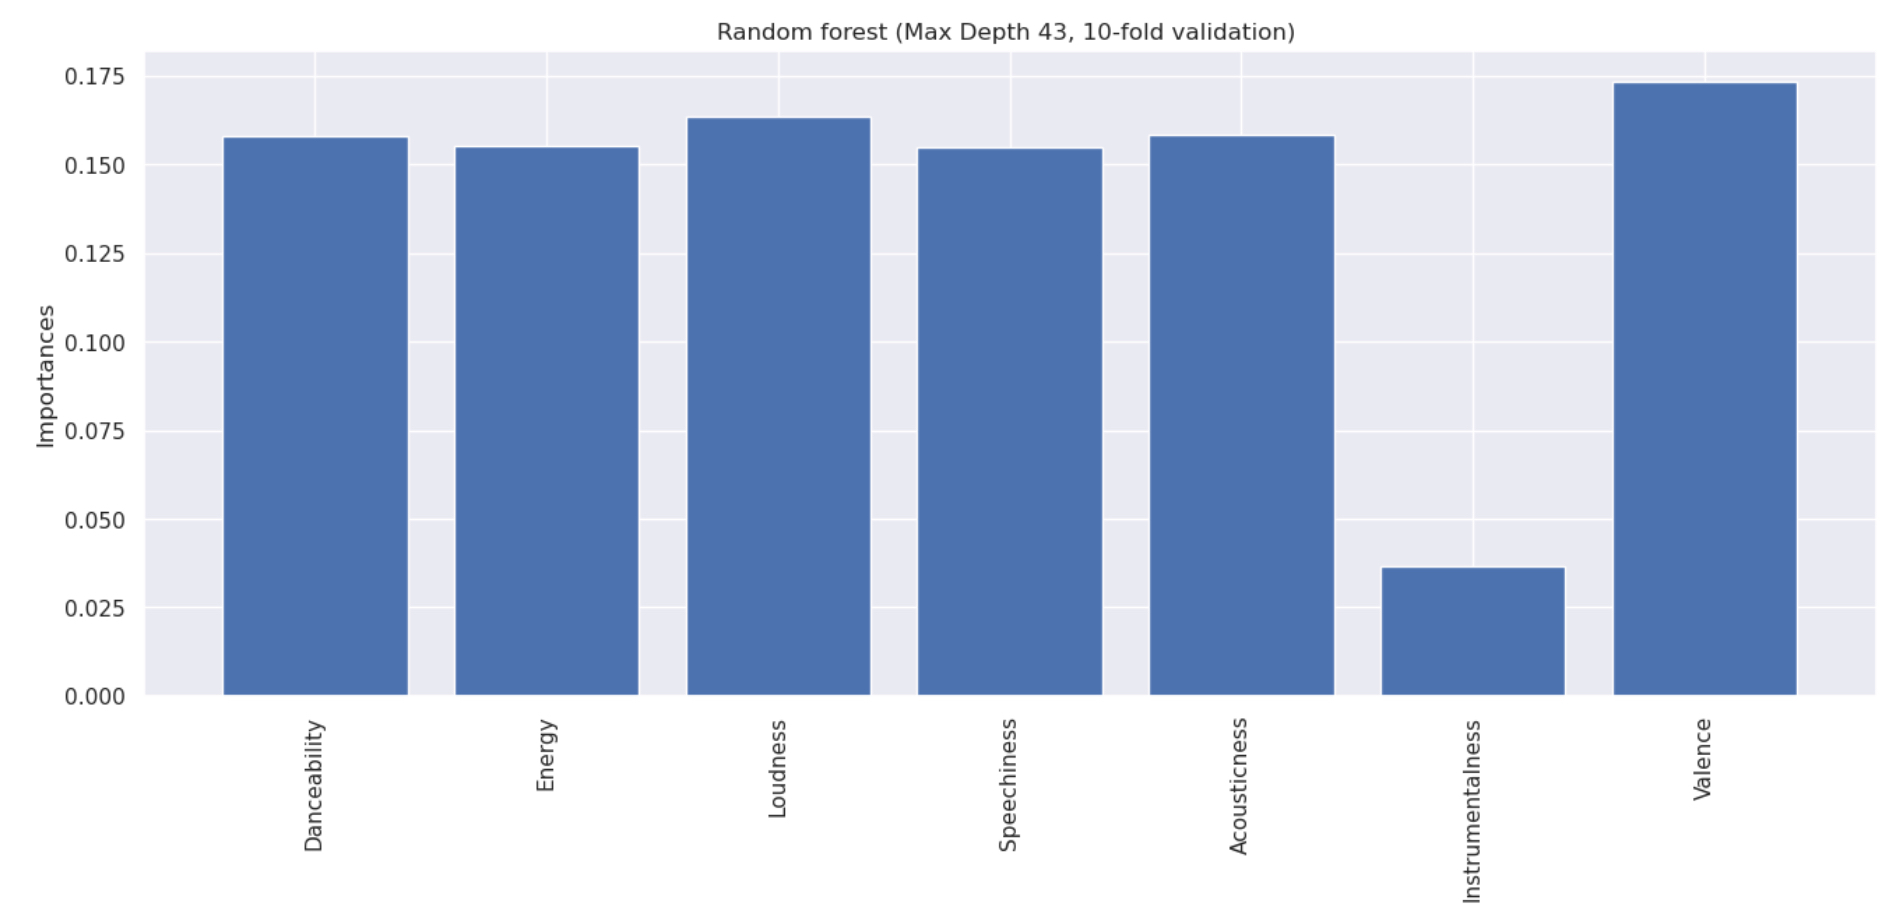
\includegraphics[width=1\linewidth]{Figures/RF_importances.png}
\end{minipage}
\caption{Comparing the importances of each feature in the DT and RF models}
\label{fig:Importances}
\end{figure}

\begin{figure}[htbp]
\centering
\begin{minipage}{1\textwidth}
  \centering
  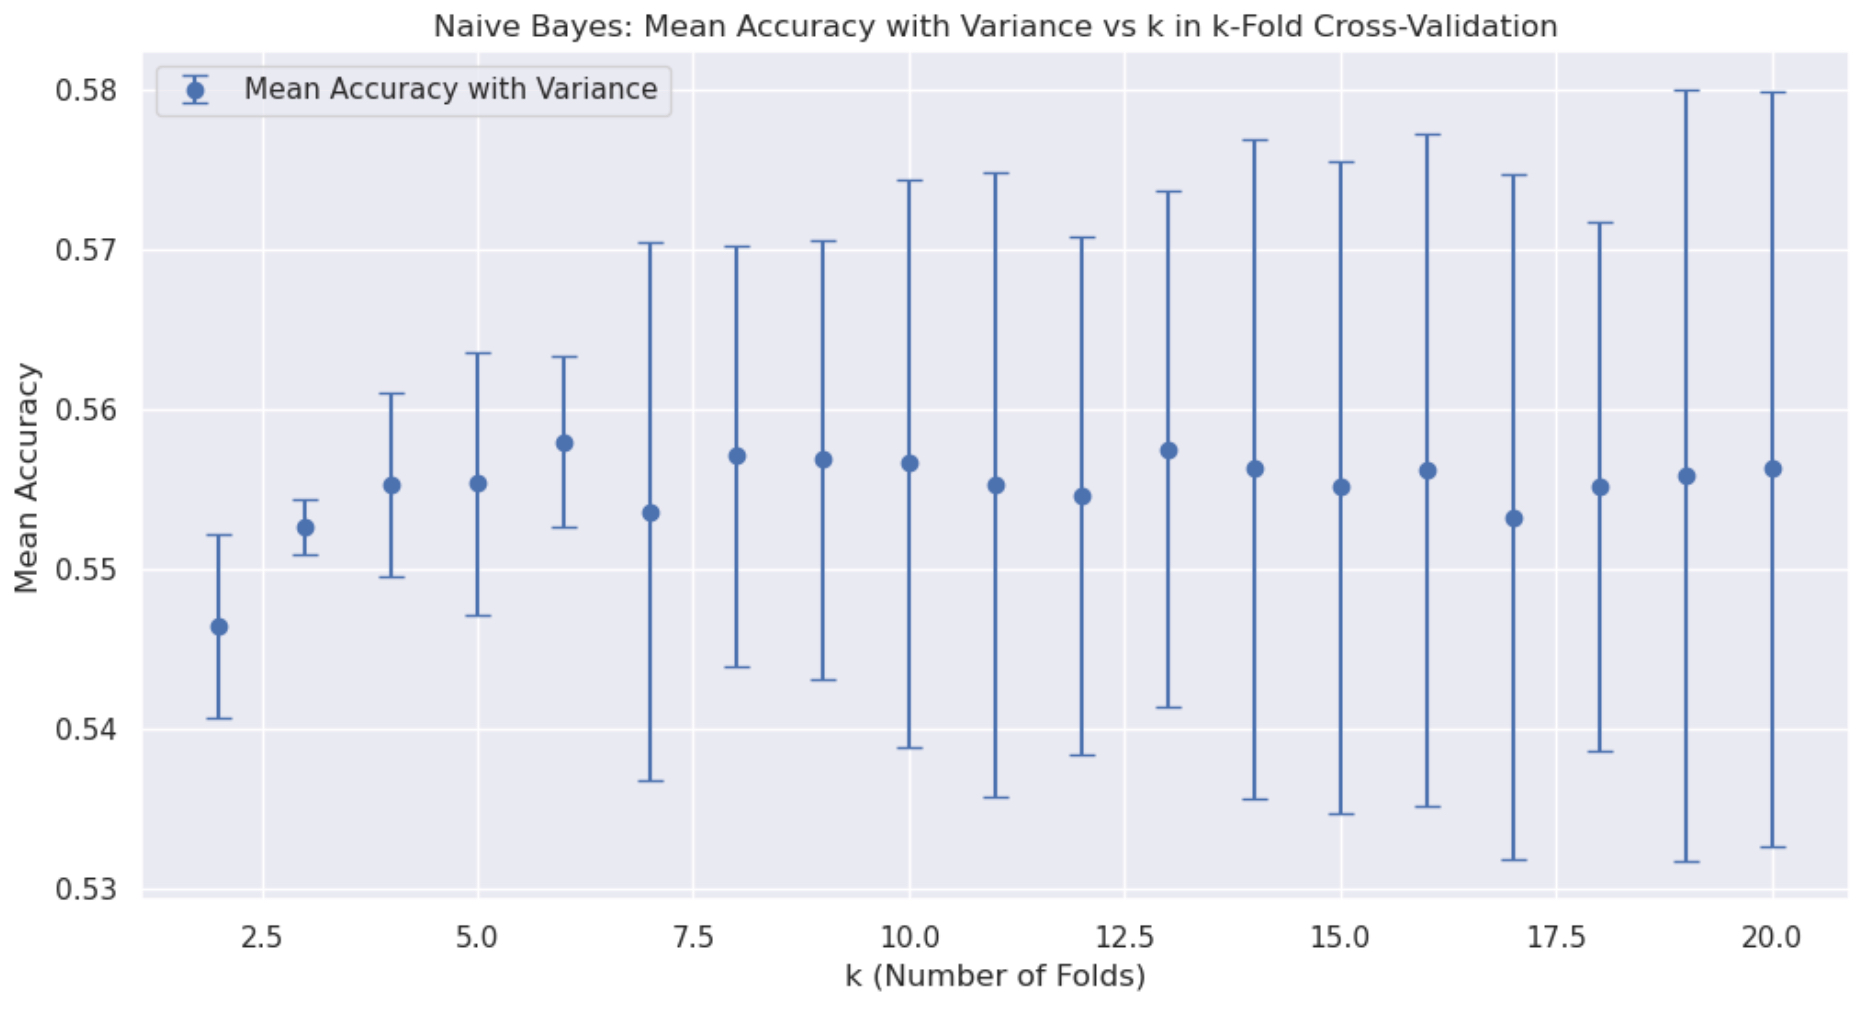
\includegraphics[width=.6\linewidth]{Figures/NB_k.png}
\end{minipage}
\begin{minipage}{1\textwidth}
  \centering
  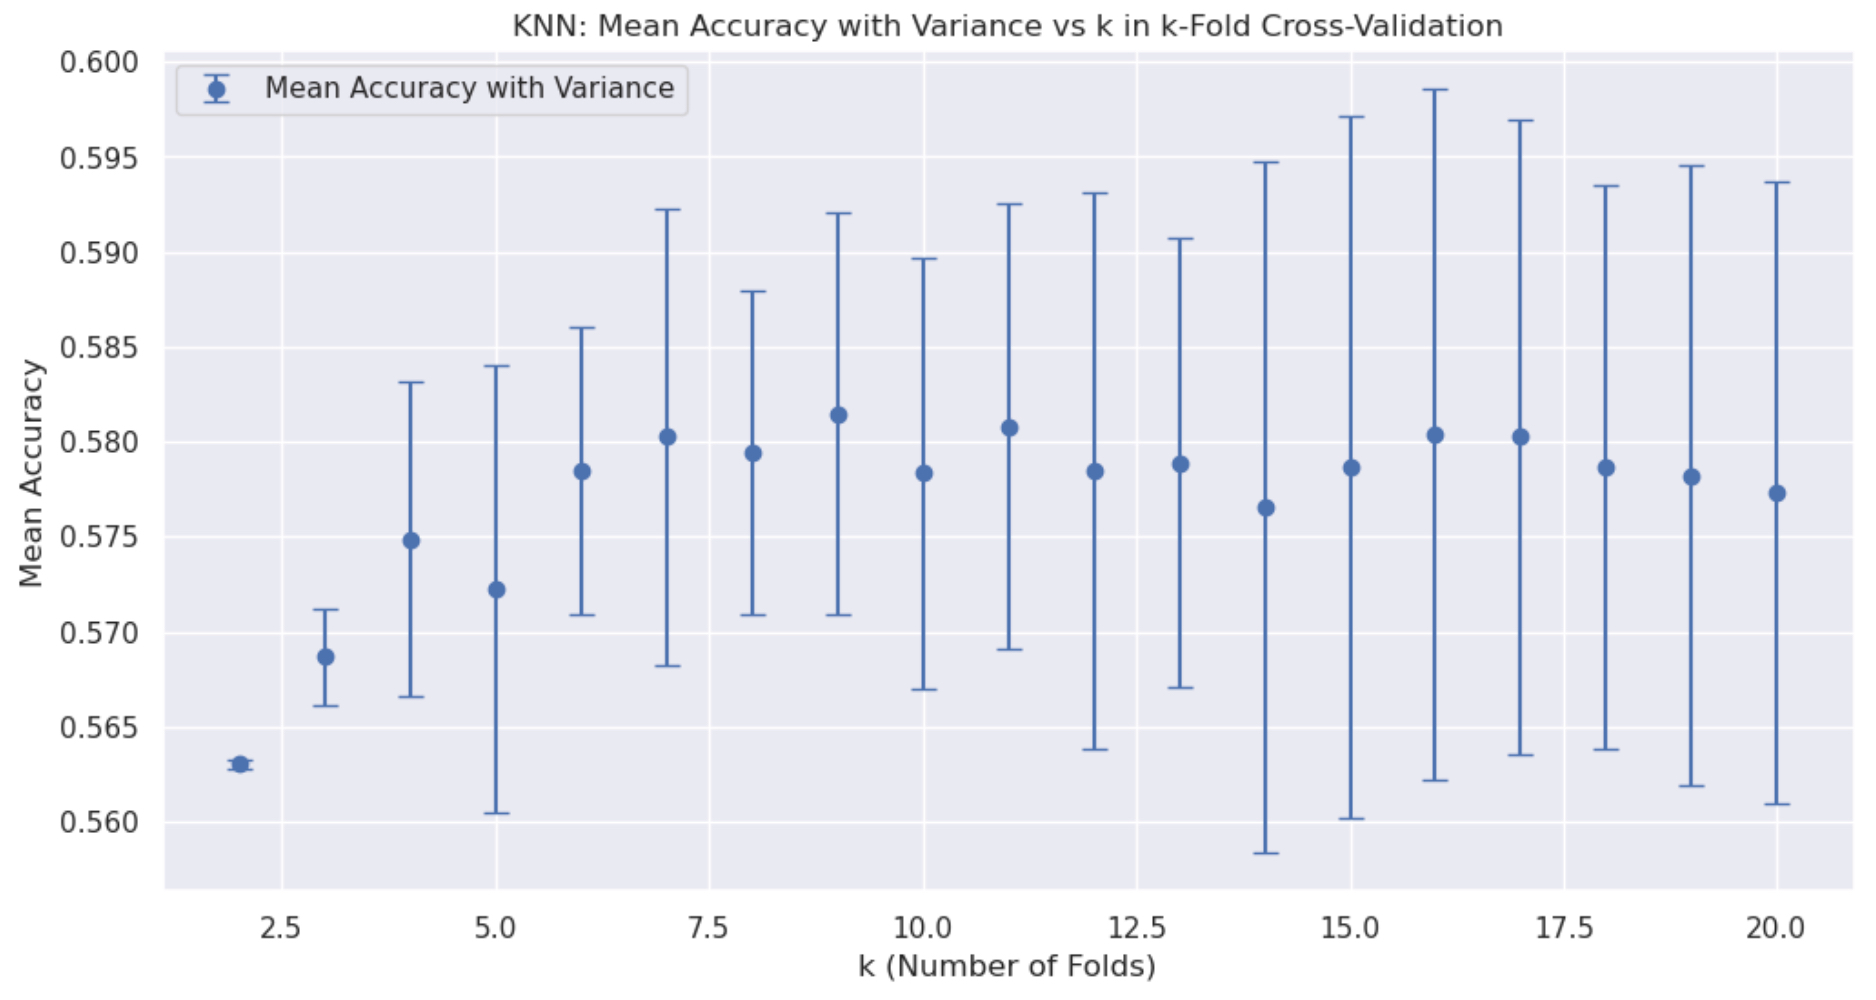
\includegraphics[width=.6\linewidth]{Figures/KNN_k.png}
\end{minipage}
\begin{minipage}{1\textwidth}
  \centering
  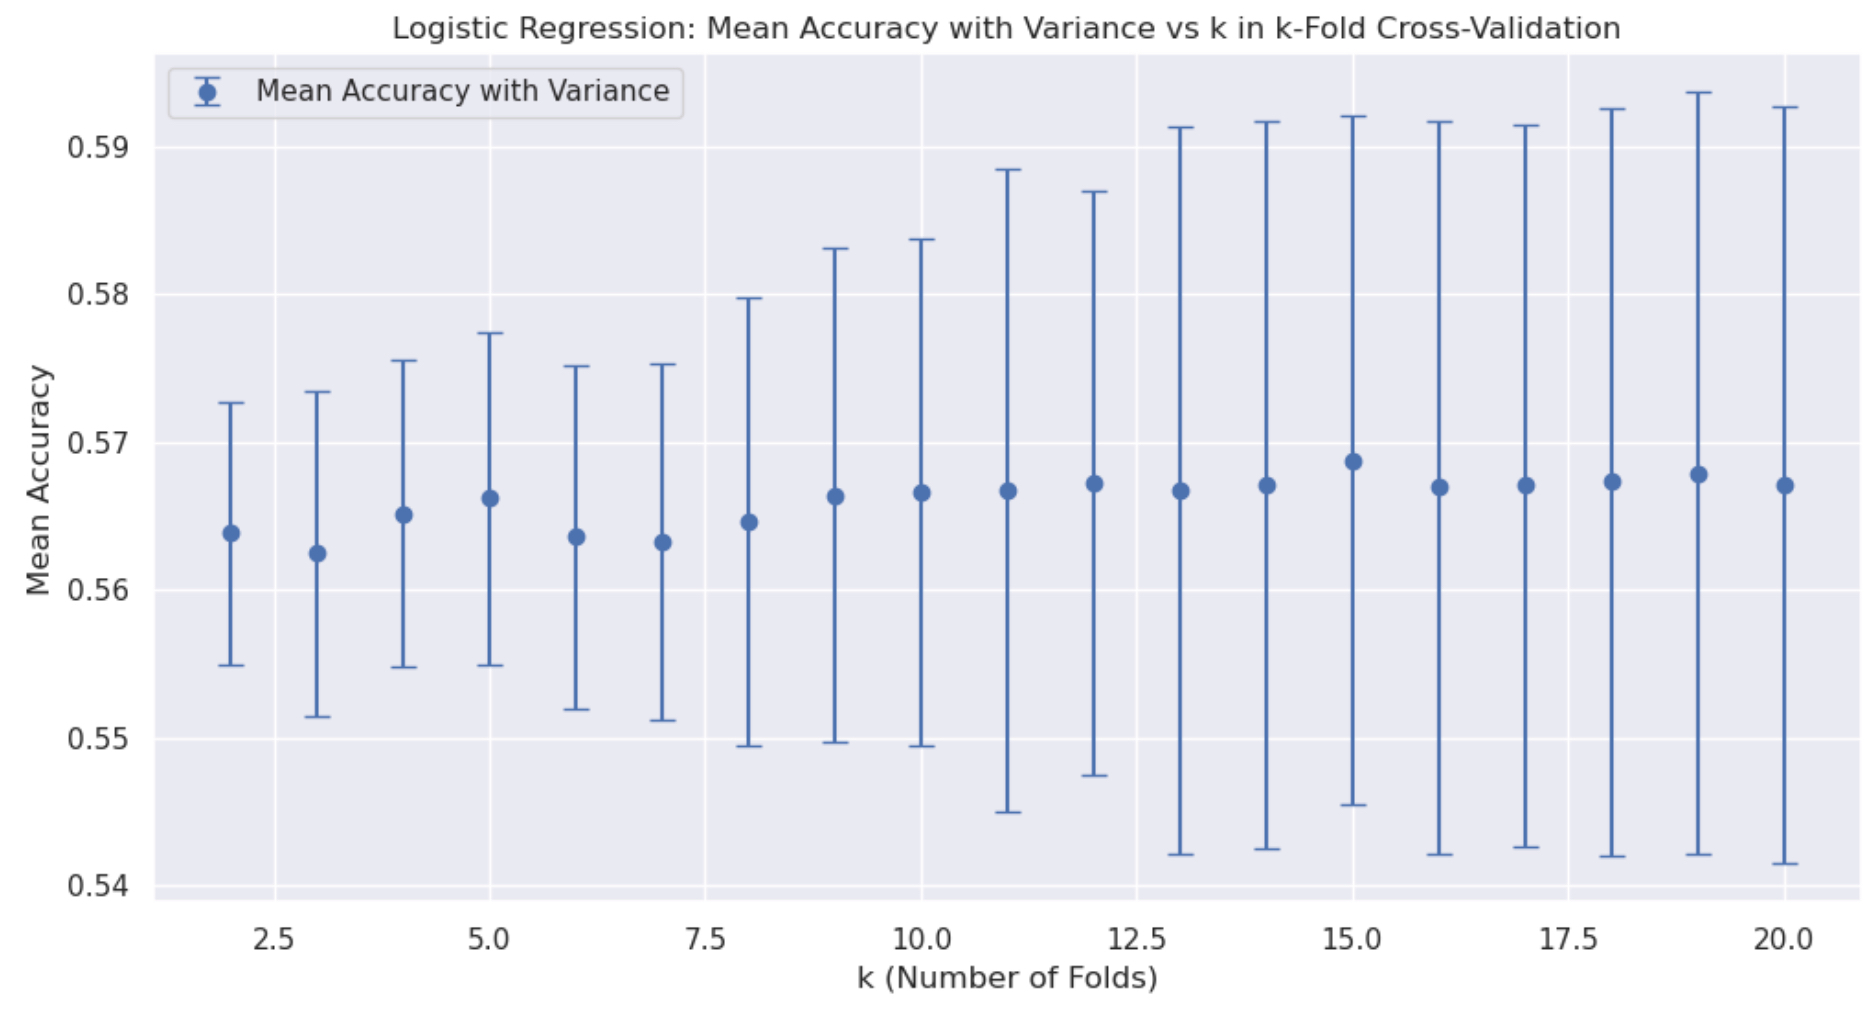
\includegraphics[width=.6\linewidth]{Figures/LR_k.png}
\end{minipage}
\begin{minipage}{1\textwidth}
  \centering
  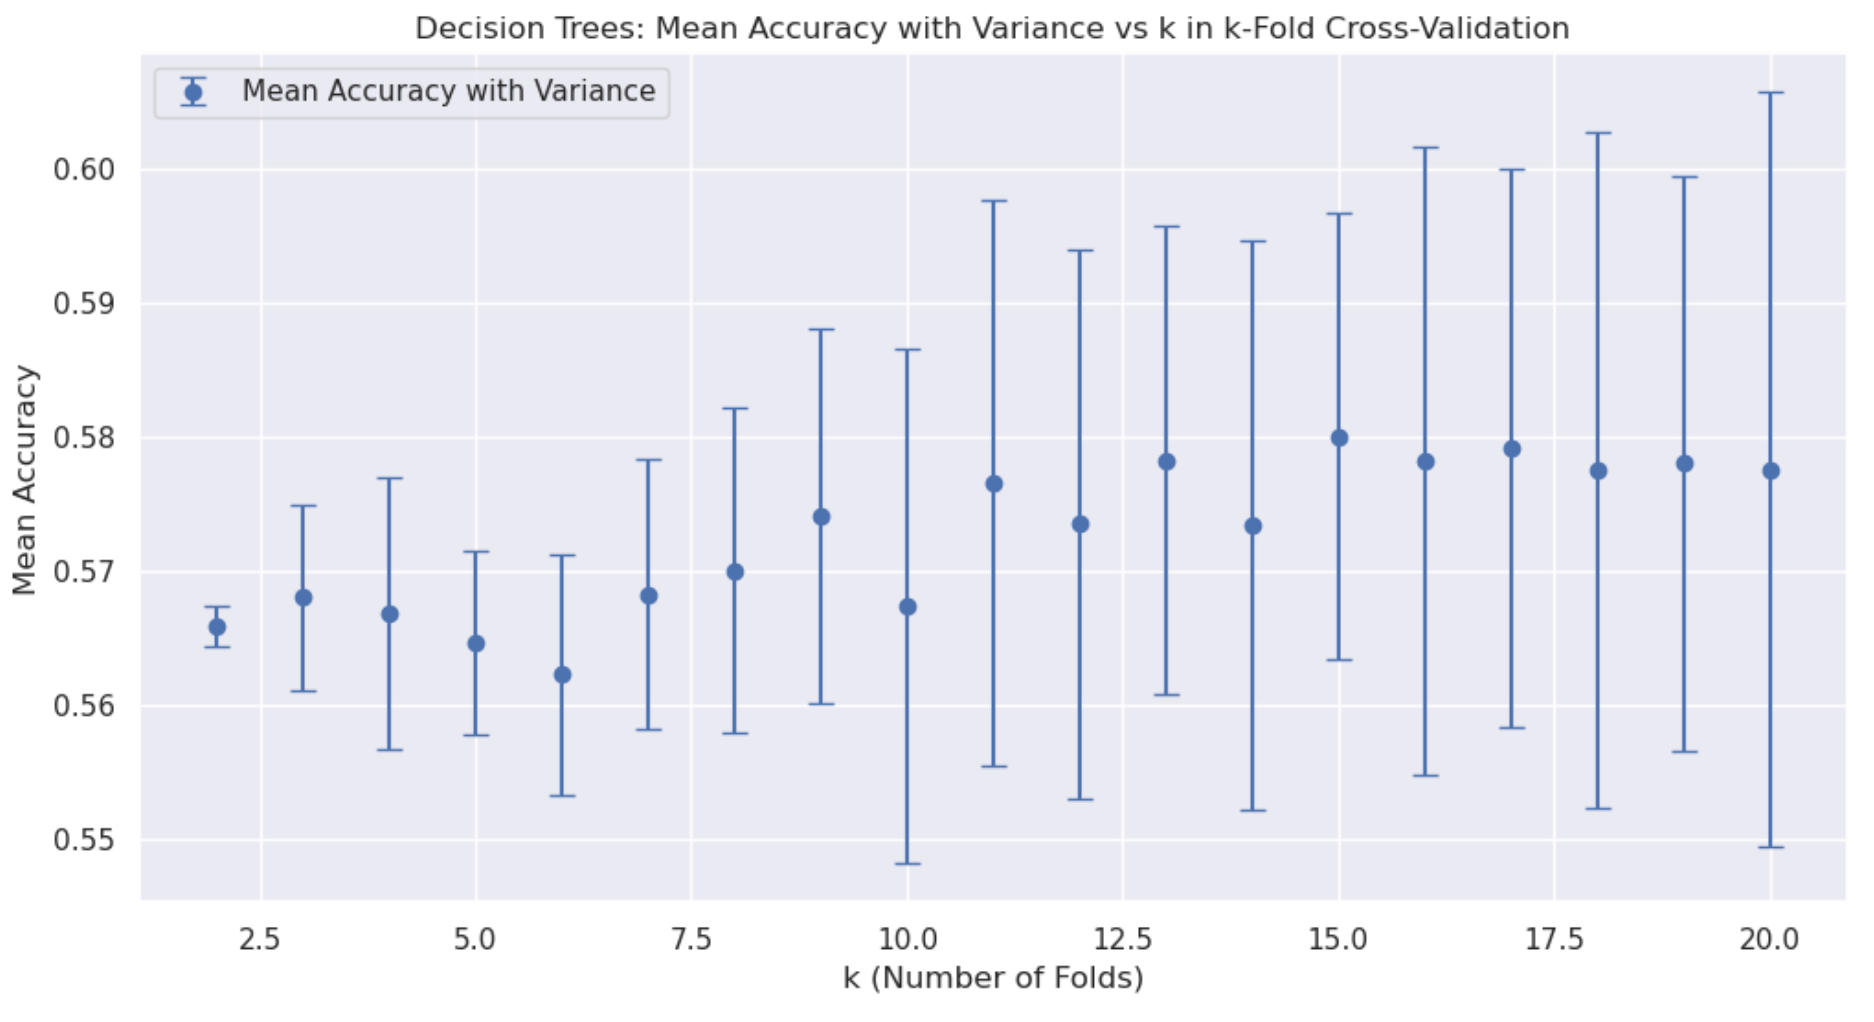
\includegraphics[width=.6\linewidth]{Figures/DT_k.png}
\end{minipage}
\begin{minipage}{1\textwidth}
  \centering
  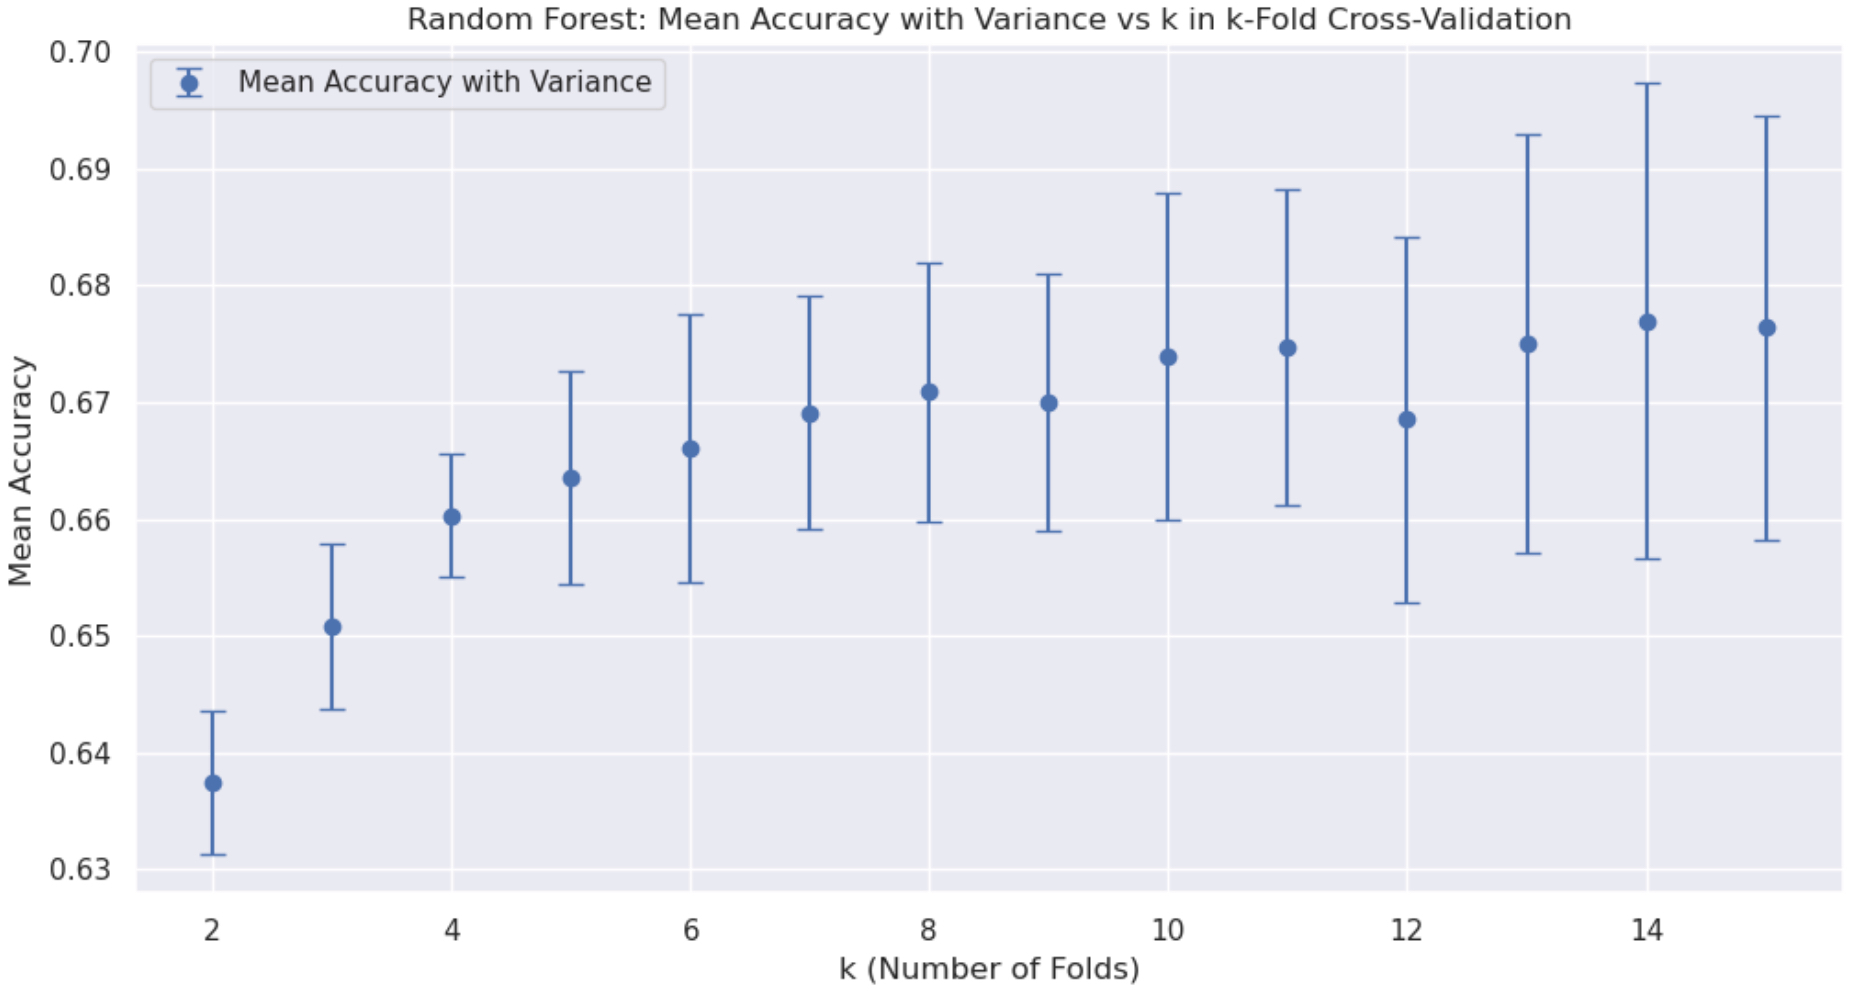
\includegraphics[width=.6\linewidth]{Figures/RF_k.png}
\end{minipage}
\caption{k-value plots for each model}
\label{fig:validation_plot}
\end{figure}

\begin{figure}[htbp]
\centering
\begin{minipage}{0.5\textwidth}
  \centering
  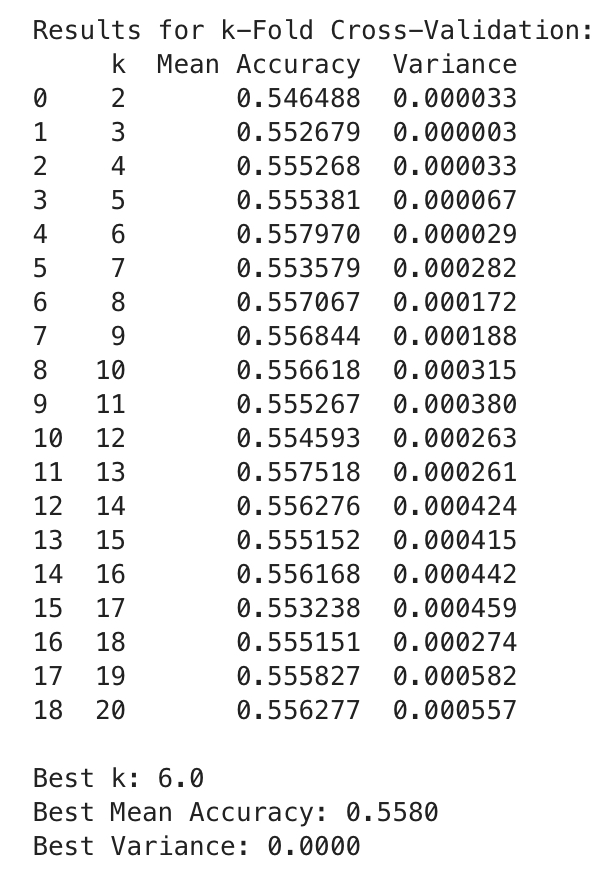
\includegraphics[width=.5\linewidth]{Figures/NB_k_list.png}
\end{minipage}%
\begin{minipage}{0.5\textwidth}
  \centering
  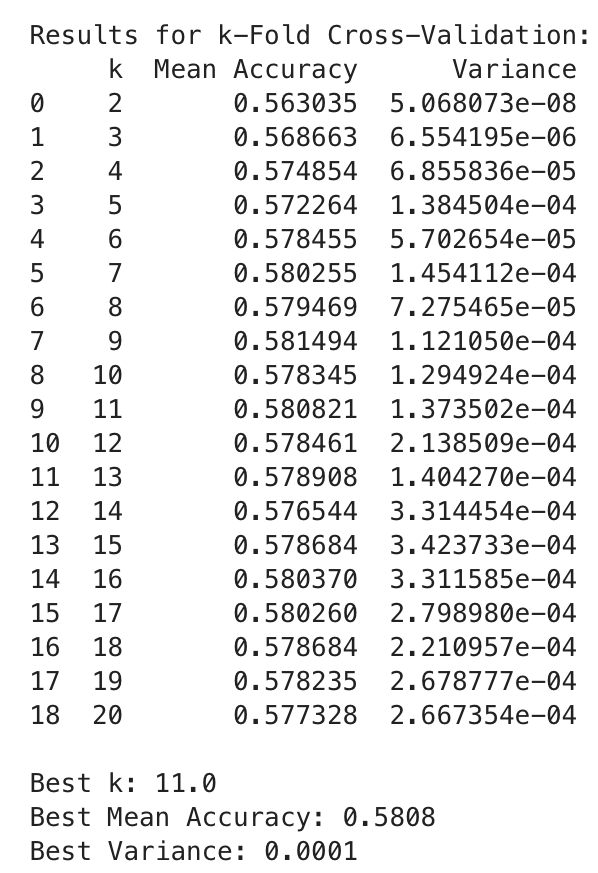
\includegraphics[width=.5\linewidth]{Figures/KNN_k_list.png}
\end{minipage}
\begin{minipage}{0.5\textwidth}
  \centering
  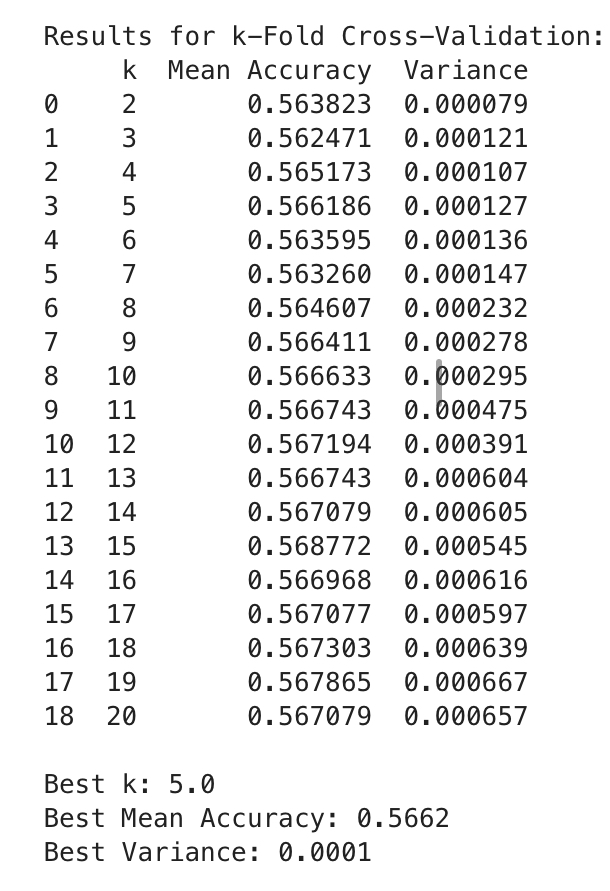
\includegraphics[width=.5\linewidth]{Figures/LR_k_list.png}
\end{minipage}%
\begin{minipage}{0.5\textwidth}
  \centering
  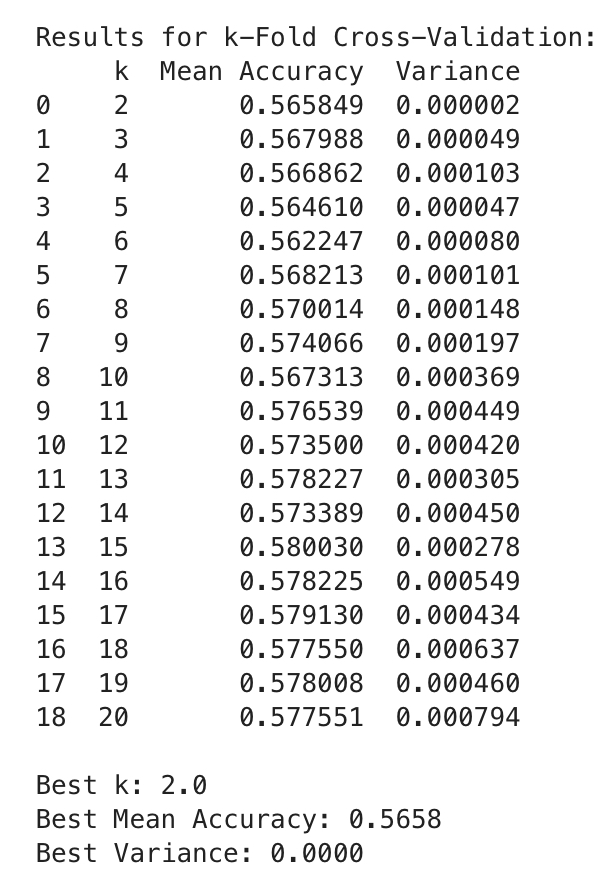
\includegraphics[width=.5\linewidth]{Figures/DT_k_list.png}
\end{minipage}
\begin{minipage}{0.5\textwidth}
  \centering
  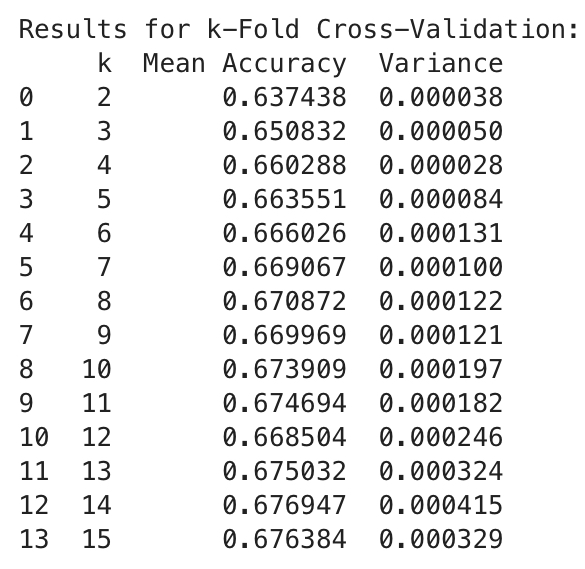
\includegraphics[width=.5\linewidth]{Figures/RF_k_list.png}
\end{minipage}
\caption{k-value tables for each model}
\label{fig:validation_table}
\end{figure}

\begin{figure}[htbp]
\centering
\begin{minipage}{1\textwidth}
  \centering
  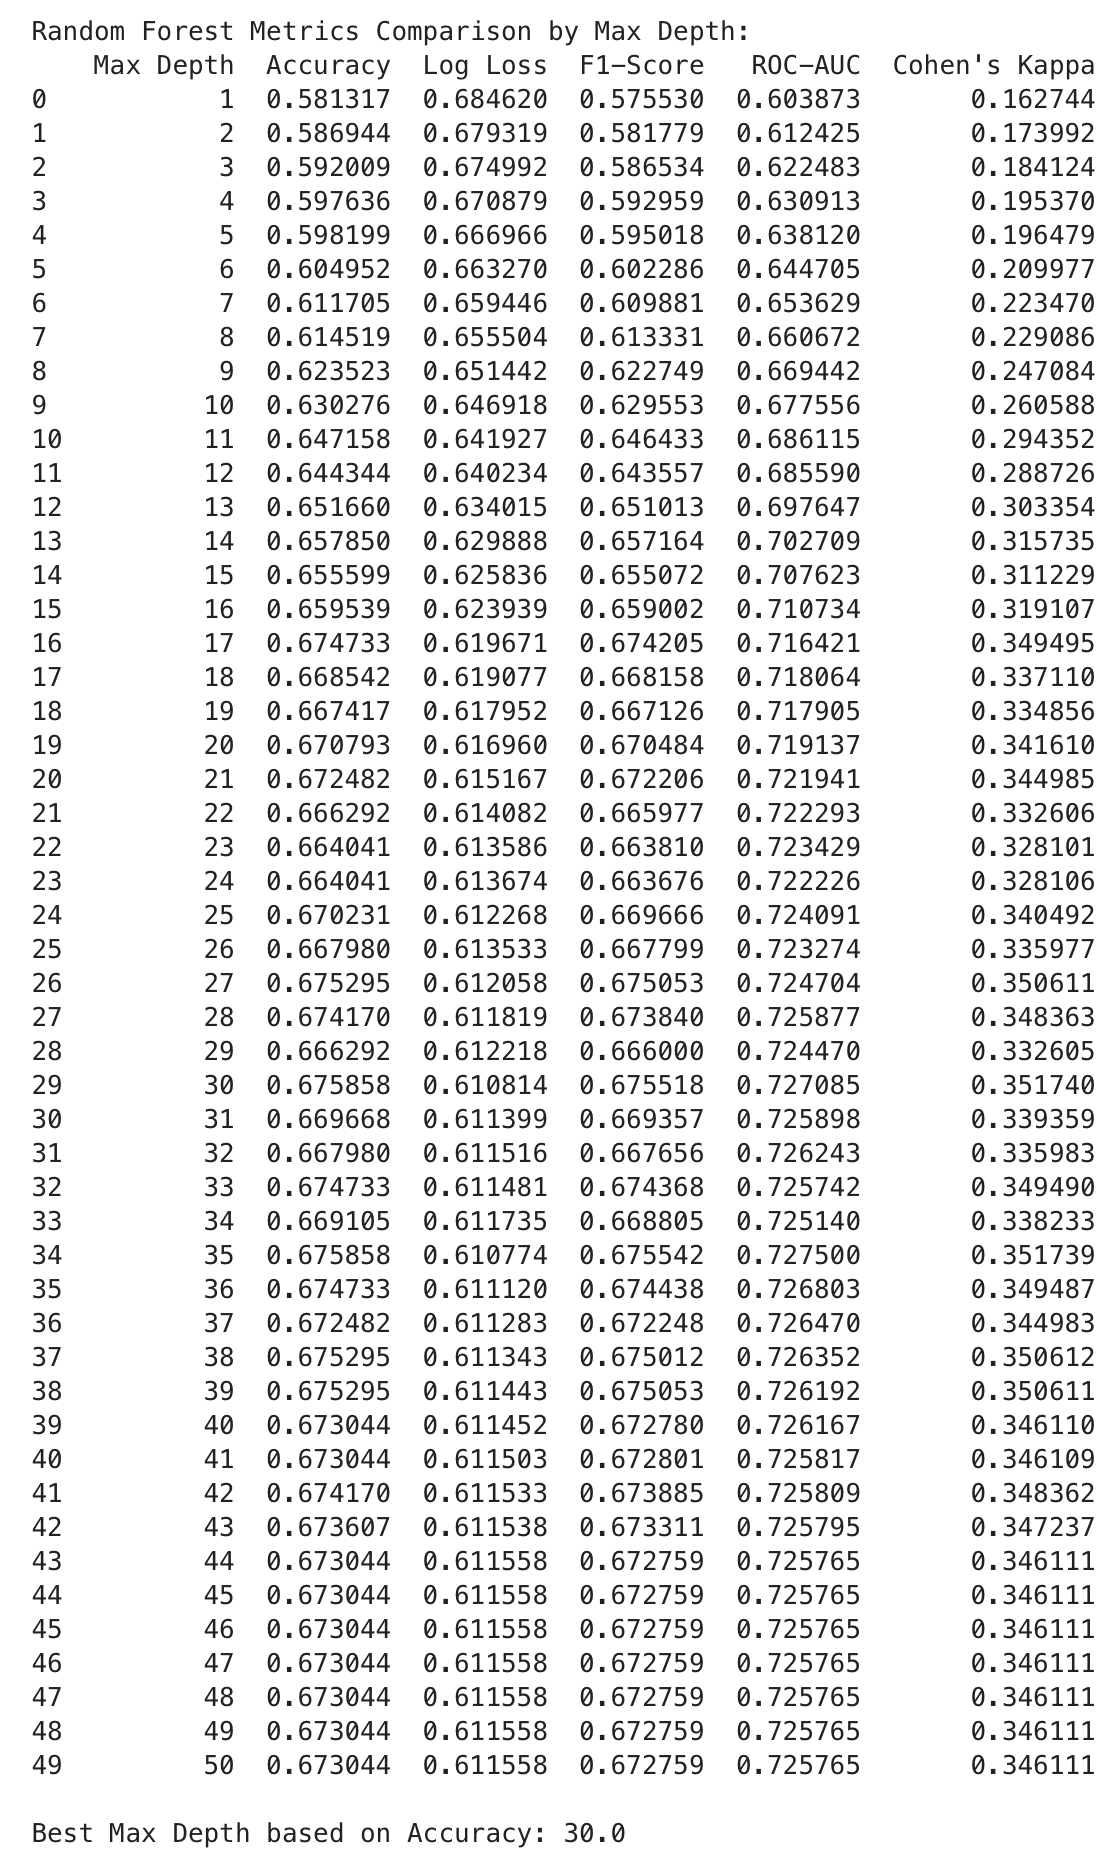
\includegraphics[width=0.5\linewidth]{Figures/RF_max_depth_list.png}
\end{minipage}
\begin{minipage}{1\textwidth}
  \centering
  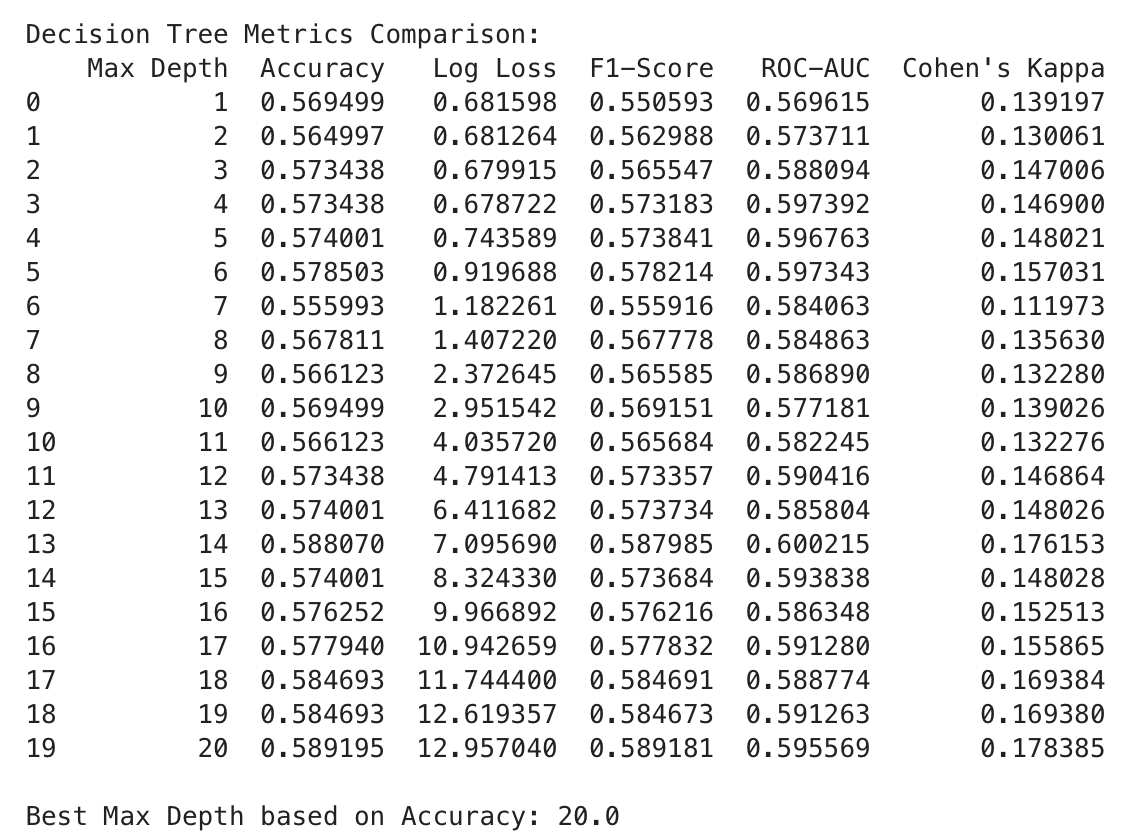
\includegraphics[width=0.5\linewidth]{Figures/DT_hyperparameter_list.png}
\end{minipage}
\begin{minipage}{1\textwidth}
  \centering
  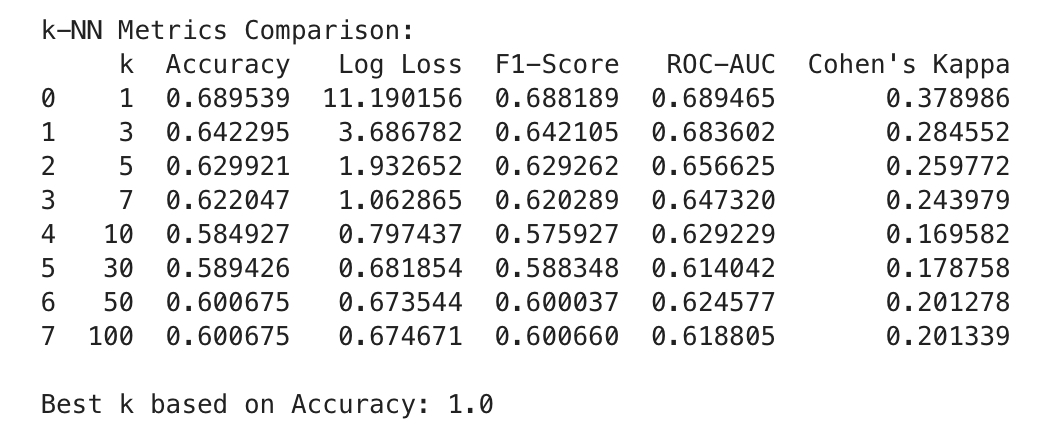
\includegraphics[width=0.5\linewidth]{Figures/KNN_hyperparameter_list.png}
\end{minipage}
\begin{minipage}{1\textwidth}
  \centering
  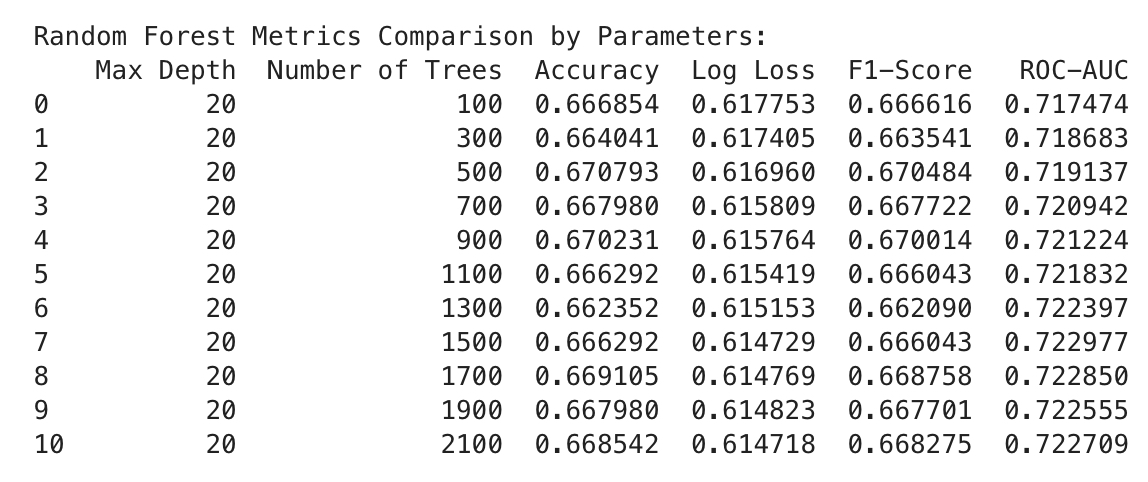
\includegraphics[width=0.5\linewidth]{Figures/RF_tree_n_list.png}
\end{minipage}
\caption{Tables of hyper-parameter performances}
\label{fig:hyperparameter_table}
\end{figure}

\begin{figure}[htbp]
\centering
\begin{minipage}{.3\textwidth}
  \centering
  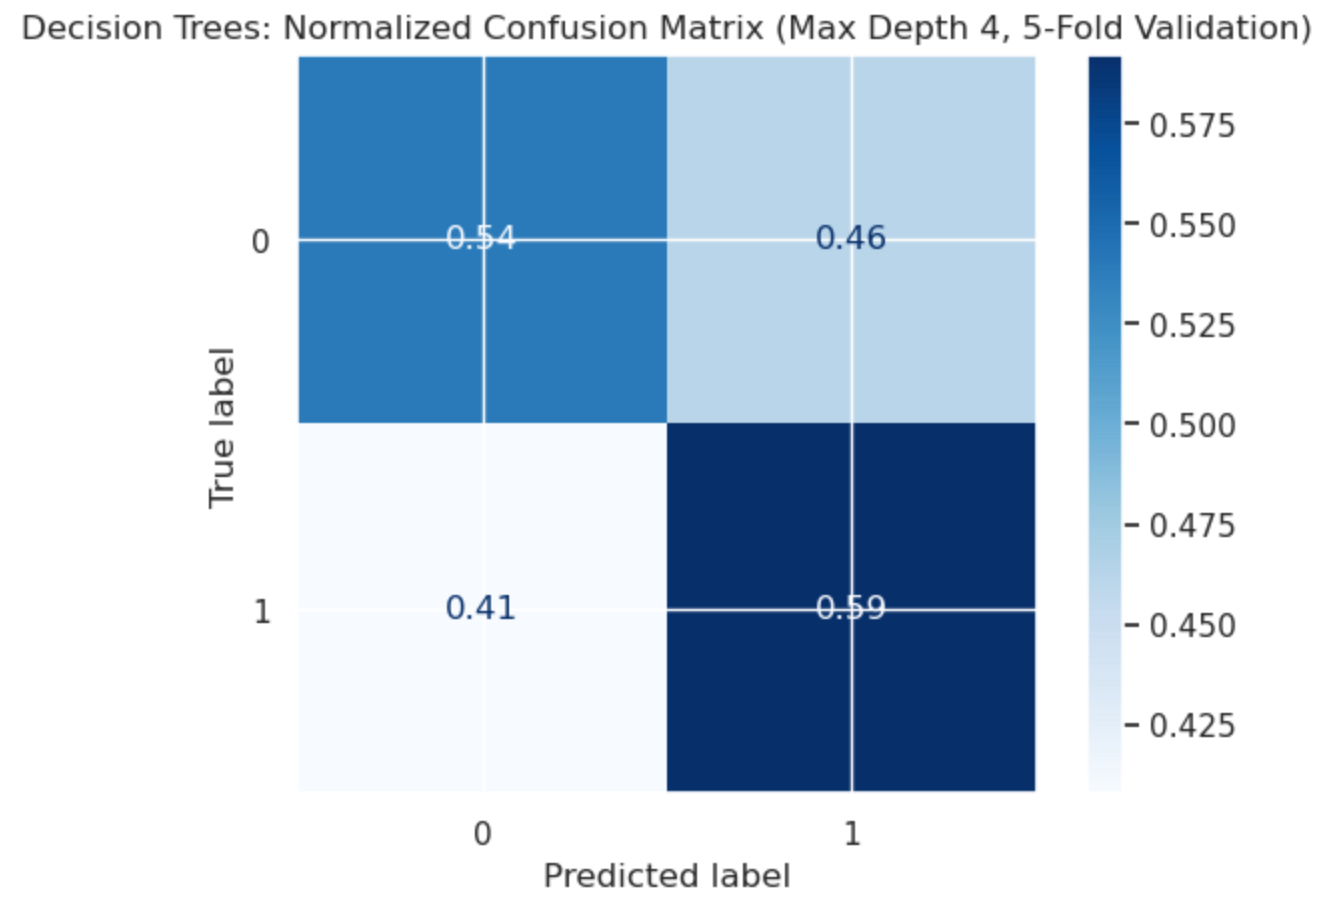
\includegraphics[width=1.03\linewidth]{Figures/DT_cm.png}
\end{minipage}%
\begin{minipage}{.3\textwidth}
  \centering
  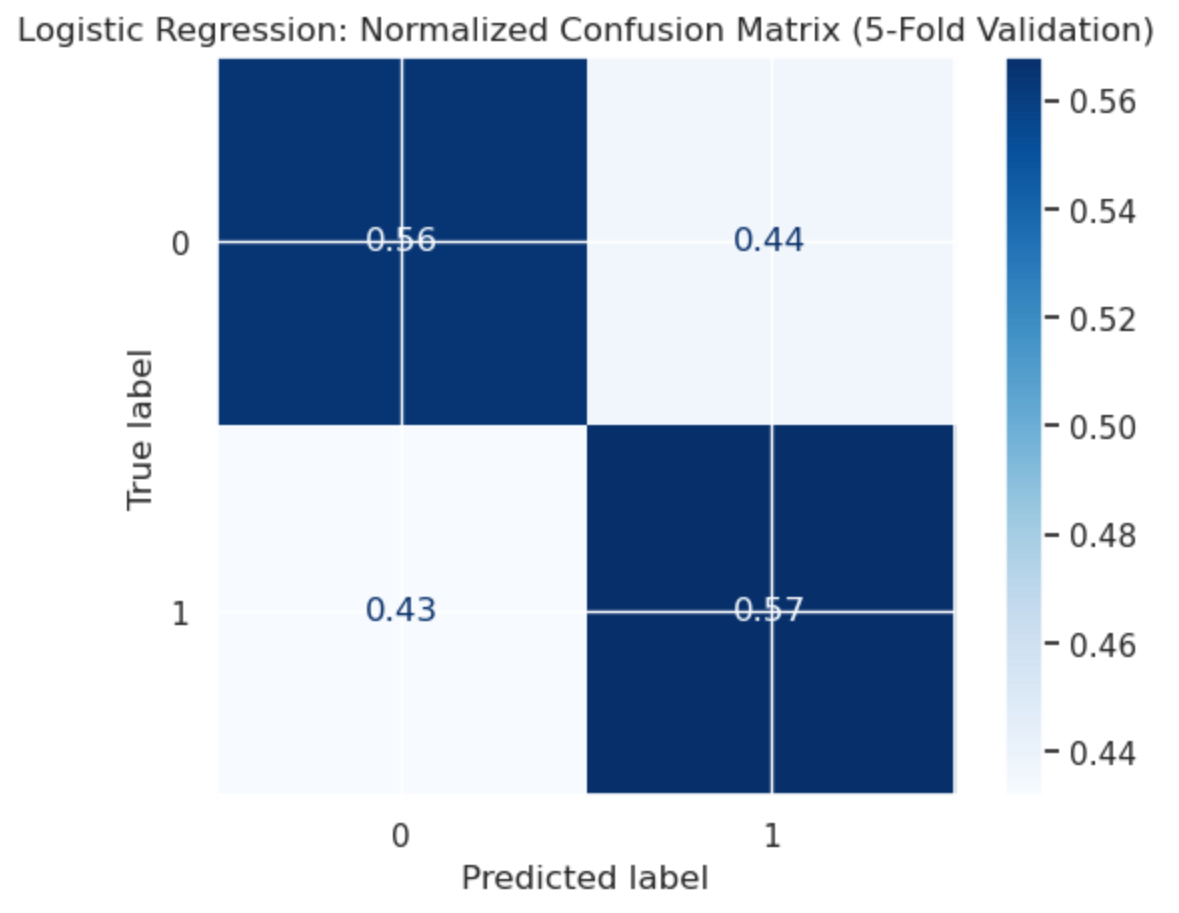
\includegraphics[width=.9\linewidth]{Figures/LR_cm.png}
\end{minipage}
\begin{minipage}{.3\textwidth}
  \centering
  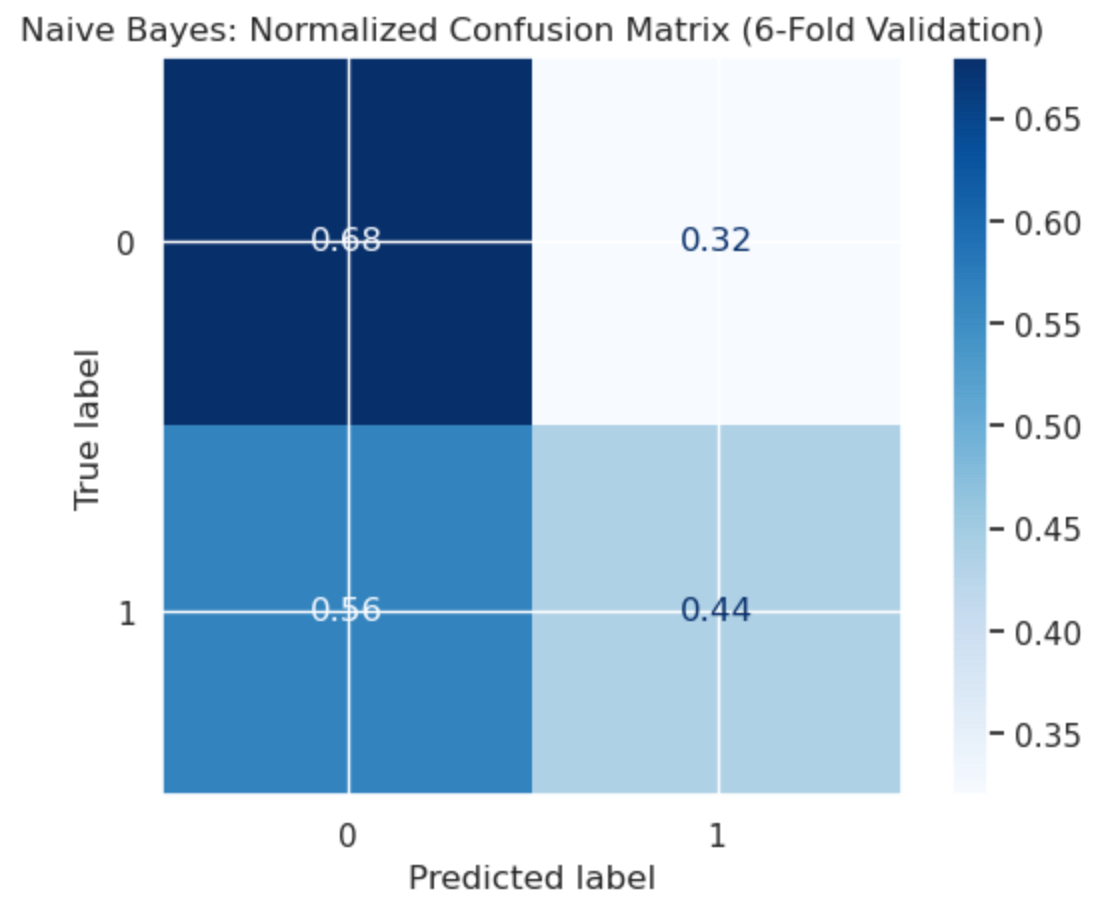
\includegraphics[width=.85\linewidth]{Figures/NB_cm.png}
\end{minipage}
\begin{minipage}{.4\textwidth}
  \centering
  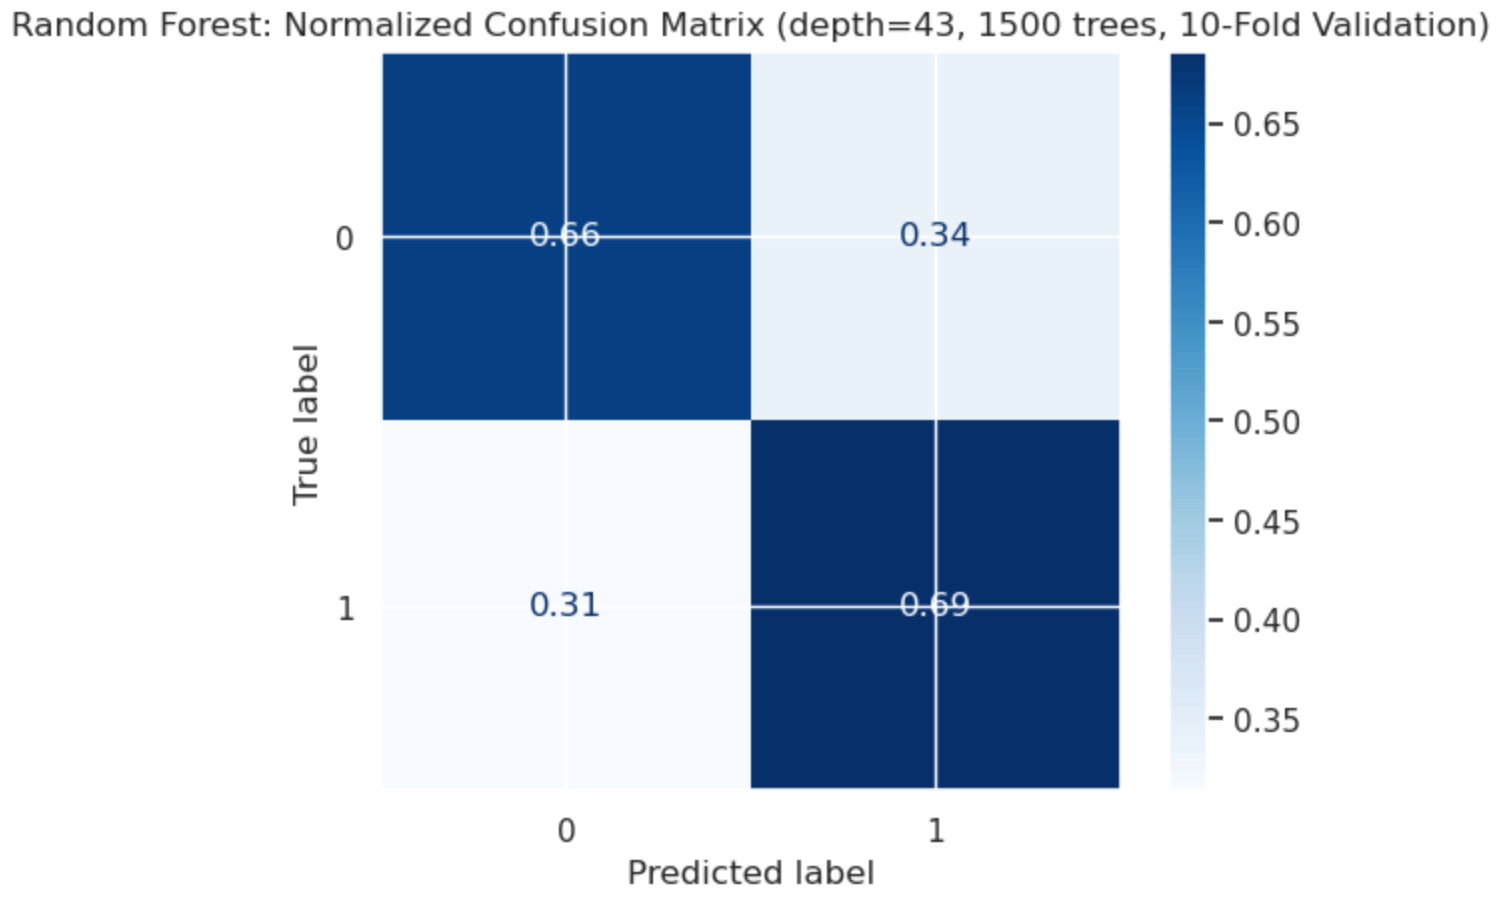
\includegraphics[width=.95\linewidth]{Figures/RF_cm.png}
\end{minipage}
\begin{minipage}{.4\textwidth}
  \centering
  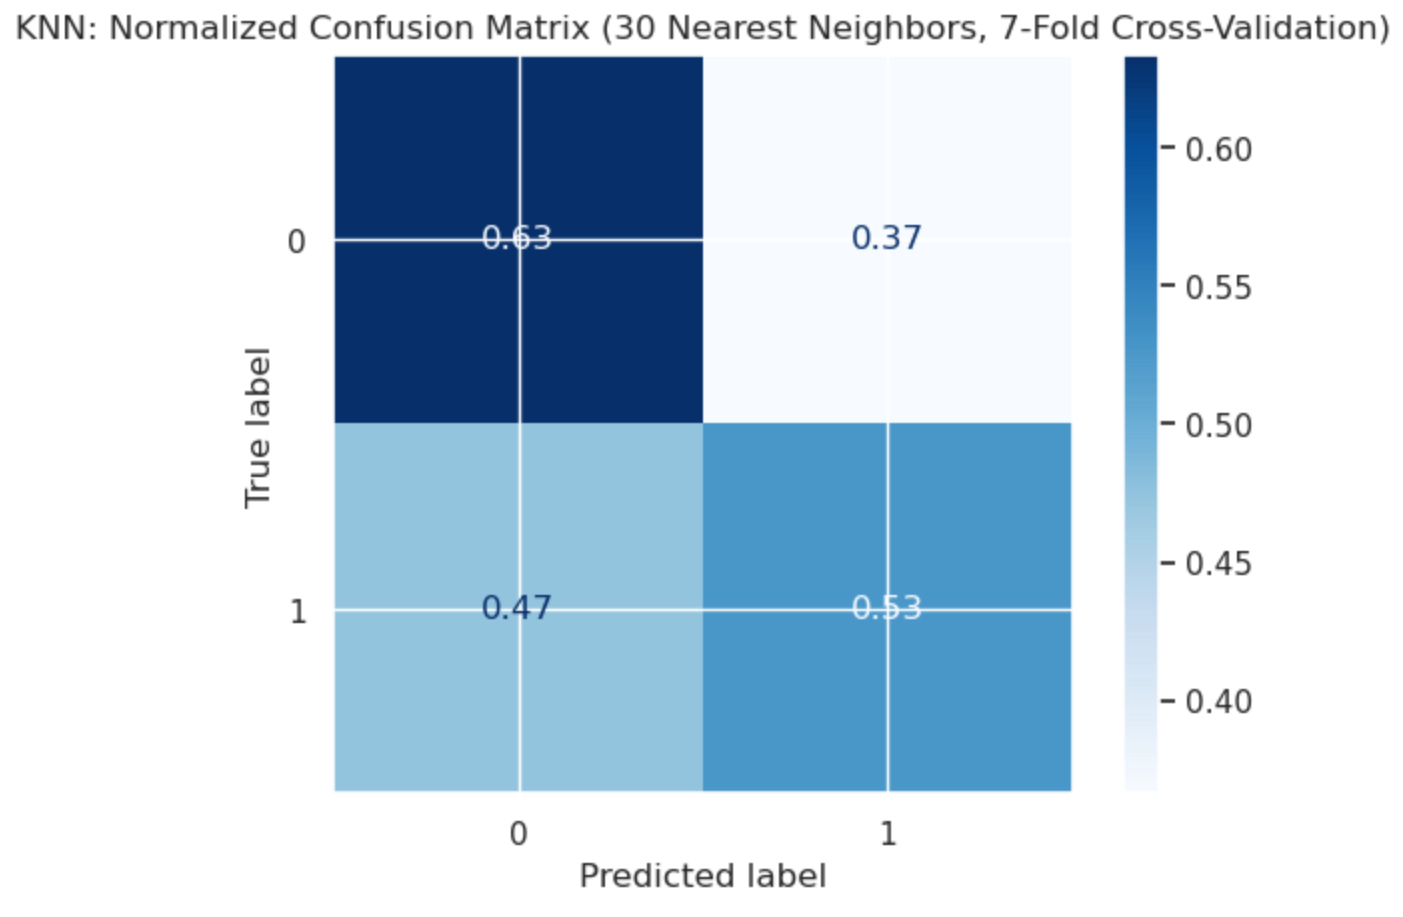
\includegraphics[width=.9\linewidth]{Figures/KNN_cm.png}
\end{minipage}
\caption{Confusion matrices of each model}
\label{fig:cm}
\end{figure}

\end{document}

%%% Local Variables:
%%% mode: latex
%%% TeX-master: t
%%% End:
